\setcounter{page}{2}

\section{Лабораторная работа №1}

\subsection{Задание для тренировки}

При создании плана проекта использовались параметры, заданные в Microsoft Project по умолчанию.
Настройки приведены на рисунке~\ref{fig:test_params}.

\begin{figure}[H]
	\centering
	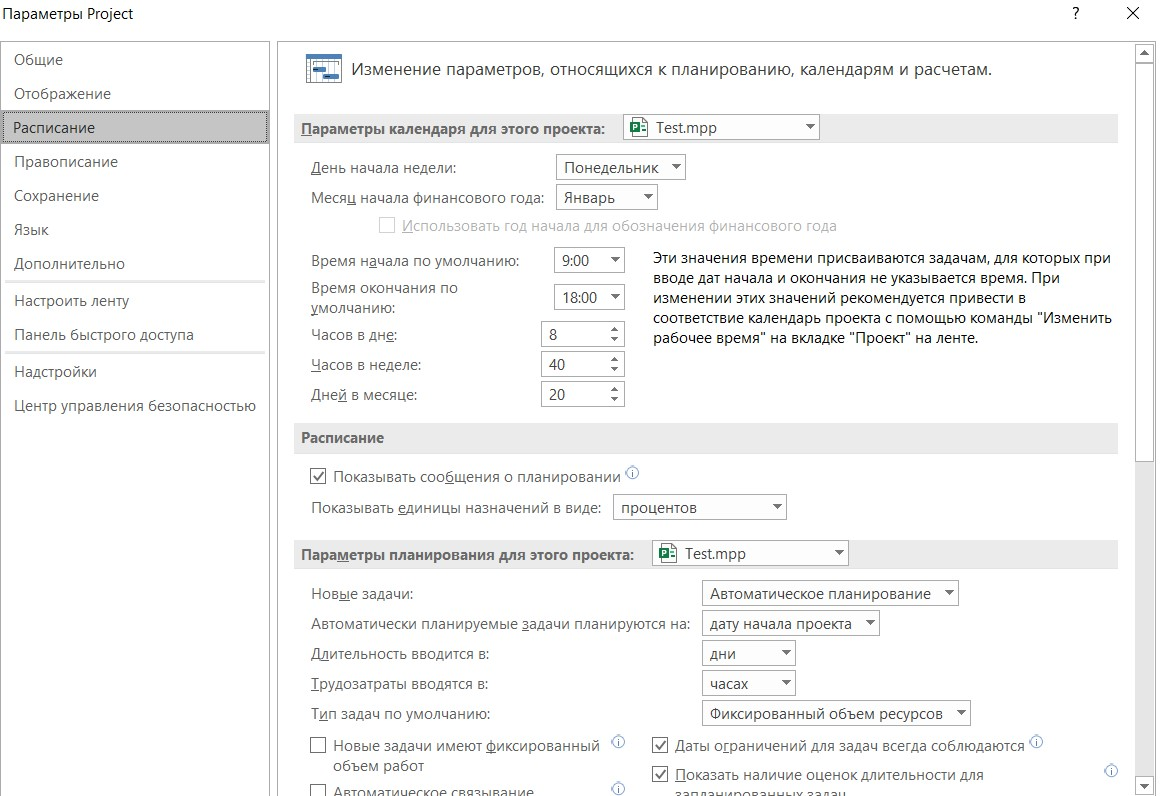
\includegraphics[width=0.9\textwidth]{img/lab1/test/params.jpg}
	\caption{Настройки проекта по умолчанию}
	\label{fig:test_params}
\end{figure}

По умолчанию рабочий день длится 8 часов с 9:00 до 18:00, в неделе 40 часов, что соответствует Трудовому кодексу.
Тип задач по умолчанию~---~с фиксированным объемом ресурсов, потому что чаще всего задано ограничение по ресурсам, а не по трудозатратам или длительности.

Датой начала проекта является первый рабочий день марта текущего года.
Настройка даты начала проекта представлена на рисунке~\ref{fig:proj_start}.

\begin{figure}[H]
	\centering
	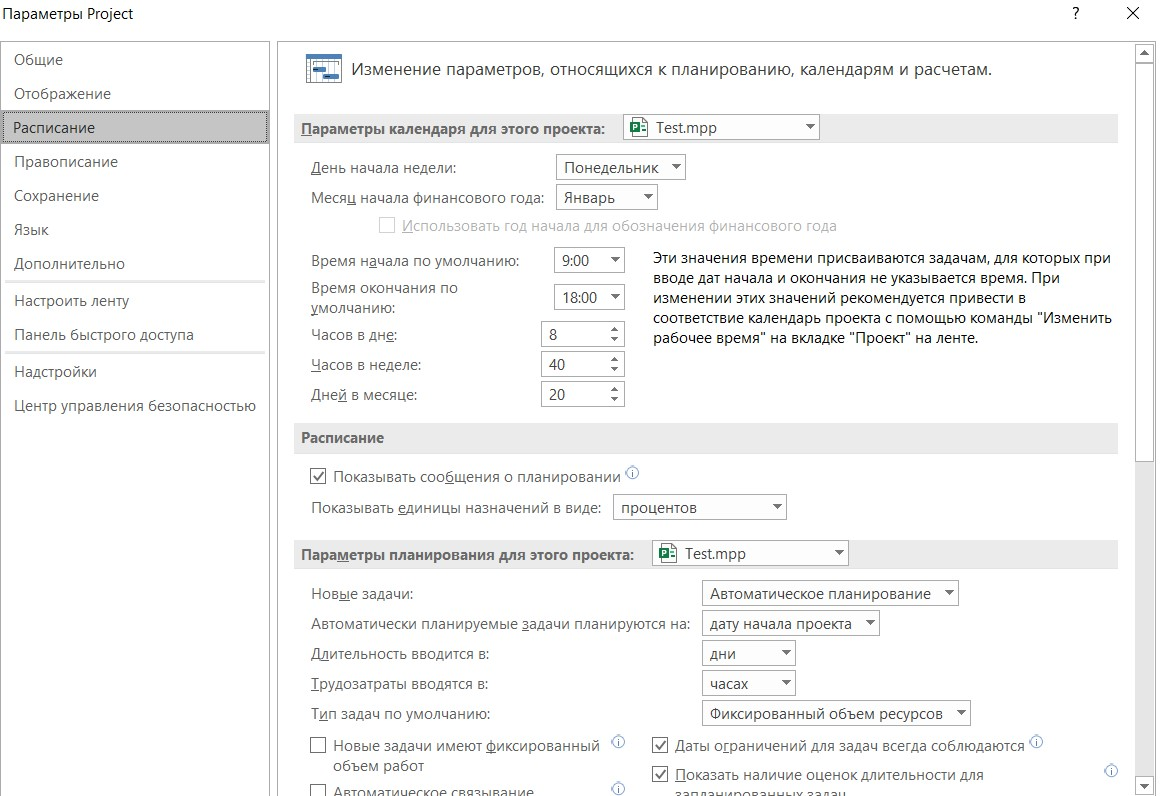
\includegraphics[width=0.9\textwidth]{img/lab1/test/params.jpg}
	\caption{Настройка даты начала проекта}
	\label{fig:proj_start}
\end{figure}

Временные характеристики проекта приведены в таблице~\ref{tbl:compare}.

\begin{table}[ht]
	\small
	\begin{center}
		\begin{threeparttable}
			\caption{Временные характеристики проекта}
			\label{tbl:compare}
			\begin{tabular}{|c|c|}
				\hline
				\textbf{Название работы}                                                & \textbf{\begin{tabular}[c]{@{}c@{}}Длительность (дни)\end{tabular}} \\ \hline
				\begin{tabular}[c]{@{}c@{}}Работа A\end{tabular}  & 12 \\ \hline
				\begin{tabular}[c]{@{}c@{}}Работа B\end{tabular}  & 6 \\ \hline
				\begin{tabular}[c]{@{}c@{}}Работа C\end{tabular}  & 10 \\ \hline
				\begin{tabular}[c]{@{}c@{}}Работа D\end{tabular}  & 7 \\ \hline
				\begin{tabular}[c]{@{}c@{}}Работа E\end{tabular}  & 9 \\ \hline
				\begin{tabular}[c]{@{}c@{}}Работа F\end{tabular}  & 8 \\ \hline
				\begin{tabular}[c]{@{}c@{}}Работа G\end{tabular}  & 10 \\ \hline
				\begin{tabular}[c]{@{}c@{}}Работа H\end{tabular}  & 10 \\ \hline
				\begin{tabular}[c]{@{}c@{}}Работа I\end{tabular}  & 6 \\ \hline
				\begin{tabular}[c]{@{}c@{}}Работа J\end{tabular}  & 5 \\ \hline
			\end{tabular}
		\end{threeparttable}
	\end{center}
\end{table}

На рисунке~\ref{fig:test} приведена построенная диаграмма Ганта.

\begin{figure}[H]
	\centering
	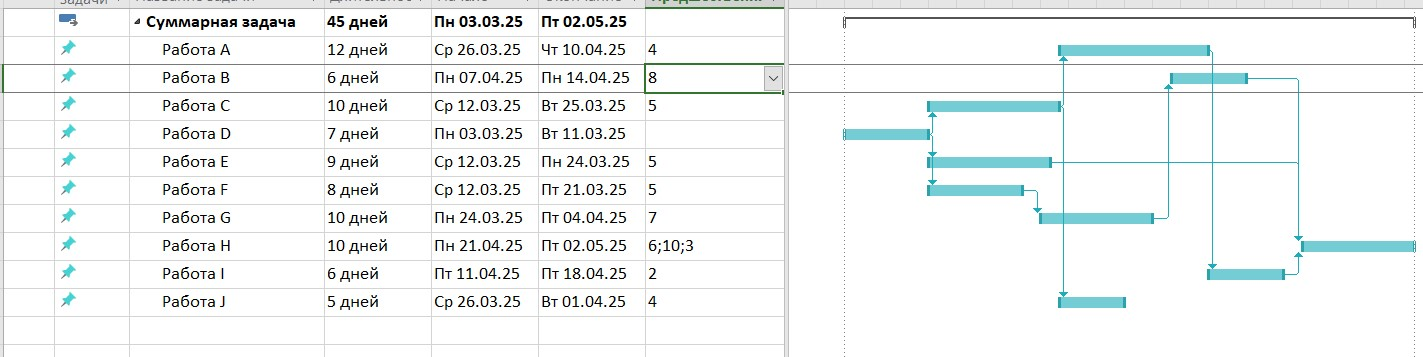
\includegraphics[width=0.9\textwidth]{img/lab1/test/test.jpg}
	\caption{Демонстрация выполнения задания для тренировки}
	\label{fig:test}
\end{figure}

Таким образом, определено, что длительность проекта для тренировки составляет 45 дней, дата его завершения~---~02.05.2025.

\subsection{Задание №1}

Проект представляет собой создание карты города.
В проекте участвуют 16 разработчиков, бюджет проекта~---~50000 рублей, длительность проекта~---~6 месяцев.
Дата начала проекта~---~первый рабочий день марта текущего года.

Перед добавлением задач необходимо настроить параметры проекта, находящиеся во вкладке $\text{Файл} \rightarrow \text{Параметры} \rightarrow \text{Расписание}$.
Настройка параметров представлена на рисунке~\ref{fig:parameters}.

\begin{figure}[H]
	\centering
	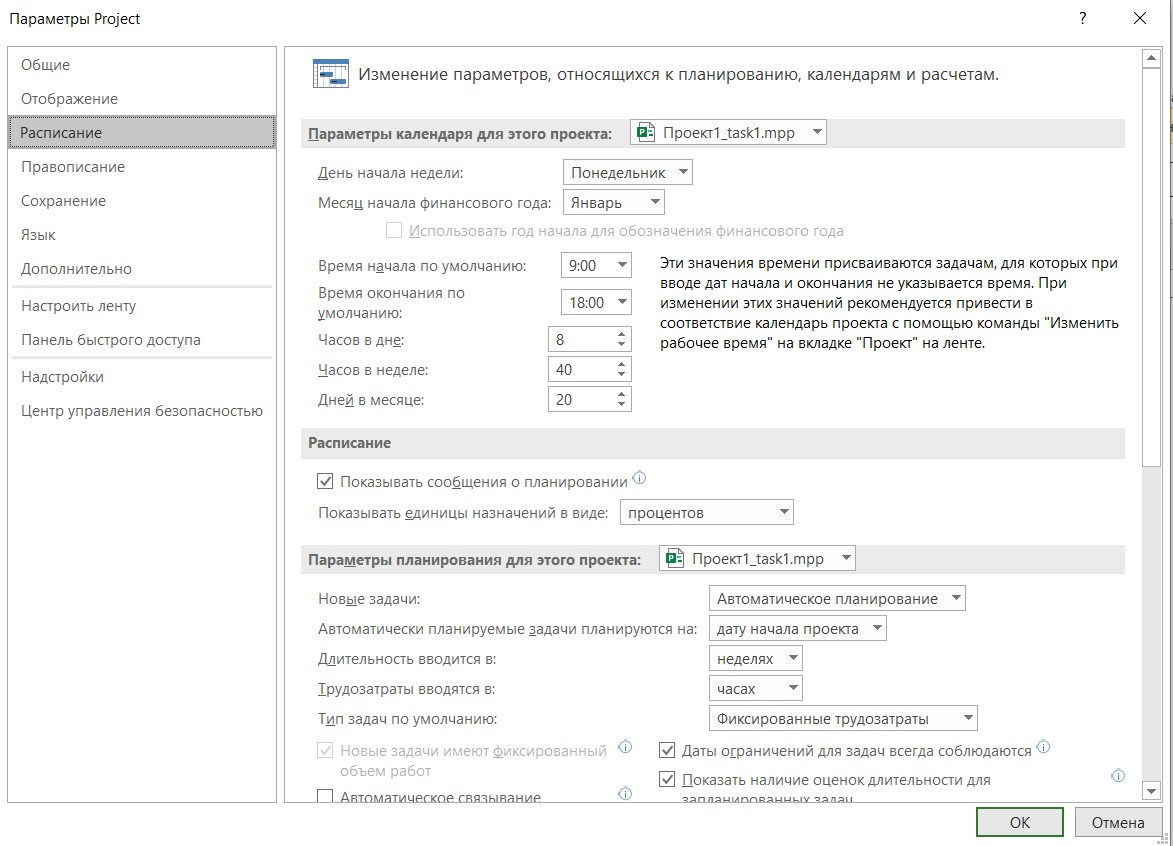
\includegraphics[width=0.9\textwidth]{img/lab1/task1/parameters.jpg}
	\caption{Настройка параметров проекта}
	\label{fig:parameters}
\end{figure}

Также необходимо внести в календарь праздничные дни и предшествующие им дни с укороченным рабочим графиком.
Для планируемого проекта такими днями являются майские праздники, день России в июне и день народного единства в ноябре.
Настройка календаря проекта приведена на рисунке~\ref{fig:calendar}.

\begin{figure}[H]
	\centering
	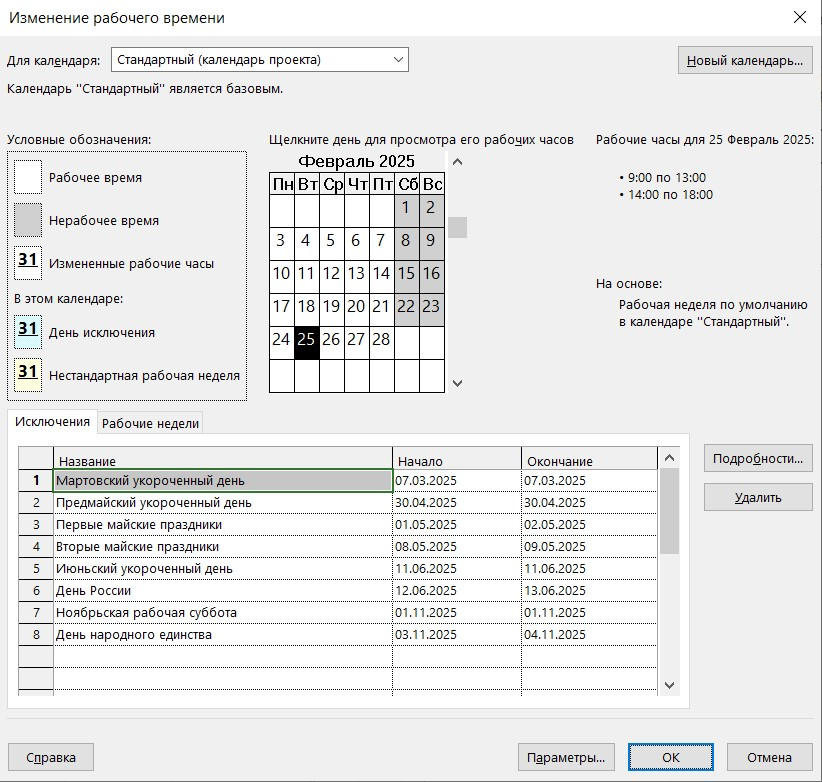
\includegraphics[width=0.9\textwidth]{img/lab1/task1/calendar.jpg}
	\caption{Настройка календаря проекта}
	\label{fig:calendar}
\end{figure}

Информацию о проекте можно посмотреть в Заметках, приведенных на рисунке~\ref{fig:notes}.

\begin{figure}[H]
	\centering
	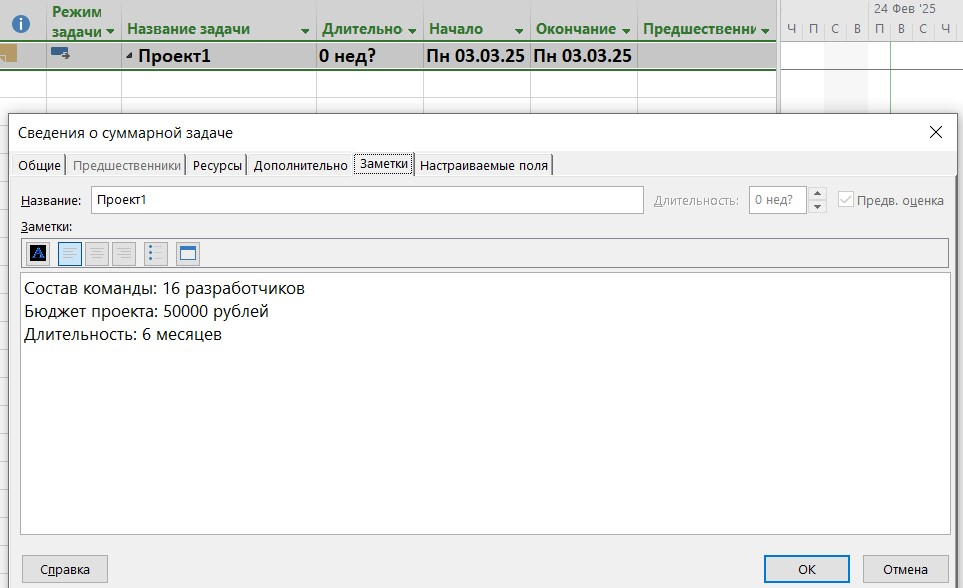
\includegraphics[width=0.9\textwidth]{img/lab1/task1/notes.jpg}
	\caption{Заметки проекта}
	\label{fig:notes}
\end{figure}

\subsection{Задание №2}

После настройки параметров проекта необходимо добавить задачи.
Так как в настройках указано, что автоматически планируемые задачи планируются на дату начала проекта, все задачи начинаются с третьего марта, что видно по диаграмме Ганта и столбцу <<Начало>> на рисунке~\ref{fig:task2}.

\begin{figure}[H]
	\centering
	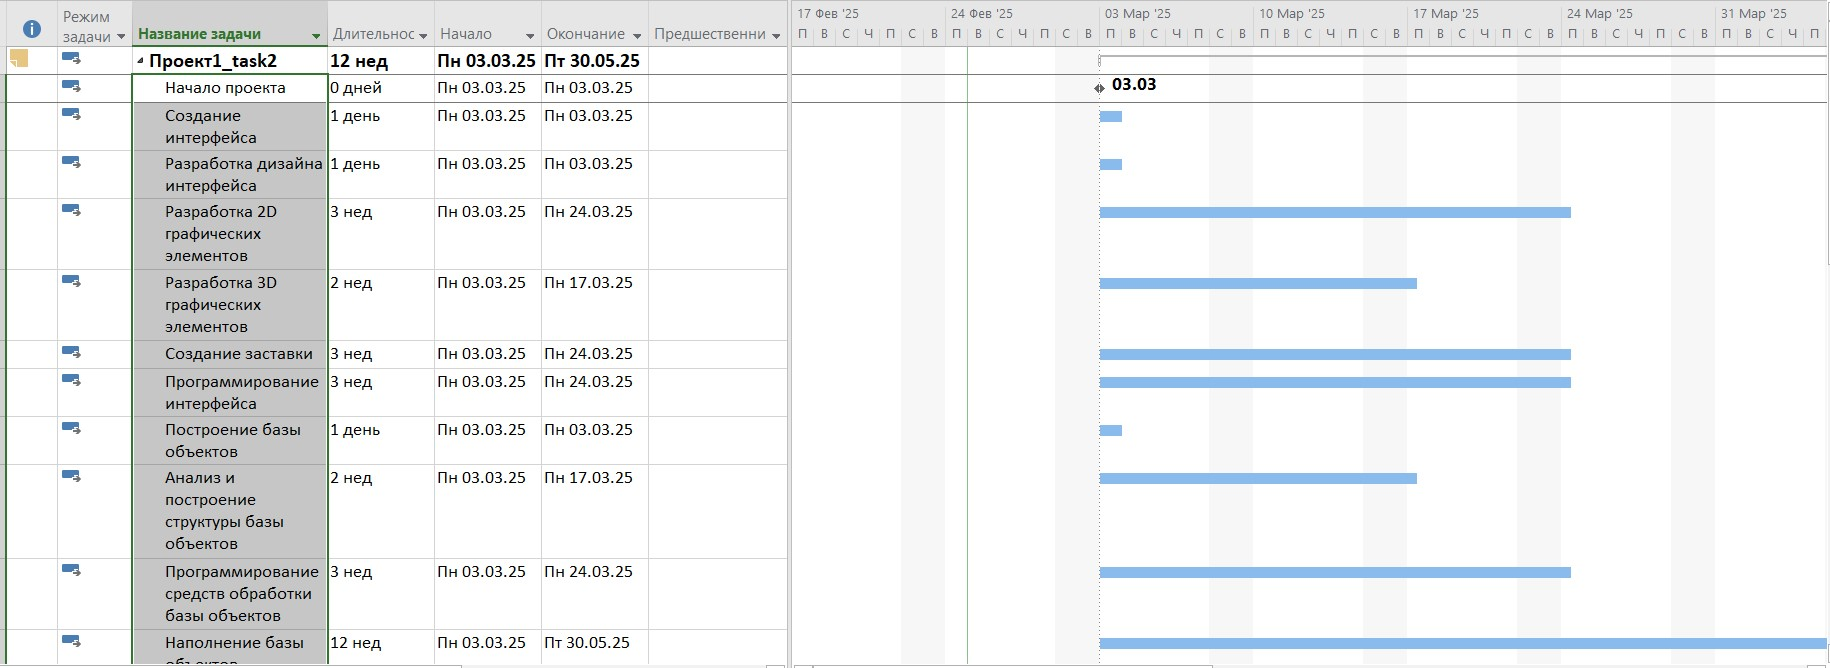
\includegraphics[width=0.9\textwidth]{img/lab1/task2/tasks.jpg}
	\caption{Диаграмма Ганта}
	\label{fig:task2}
\end{figure}

\subsection{Задание №3}

При проведении структурирования списка задач были выделены фазы проекта.
Результат структурирования списка задач приведен на рисунке~\ref{fig:task3}.

\begin{figure}[H]
	\centering
	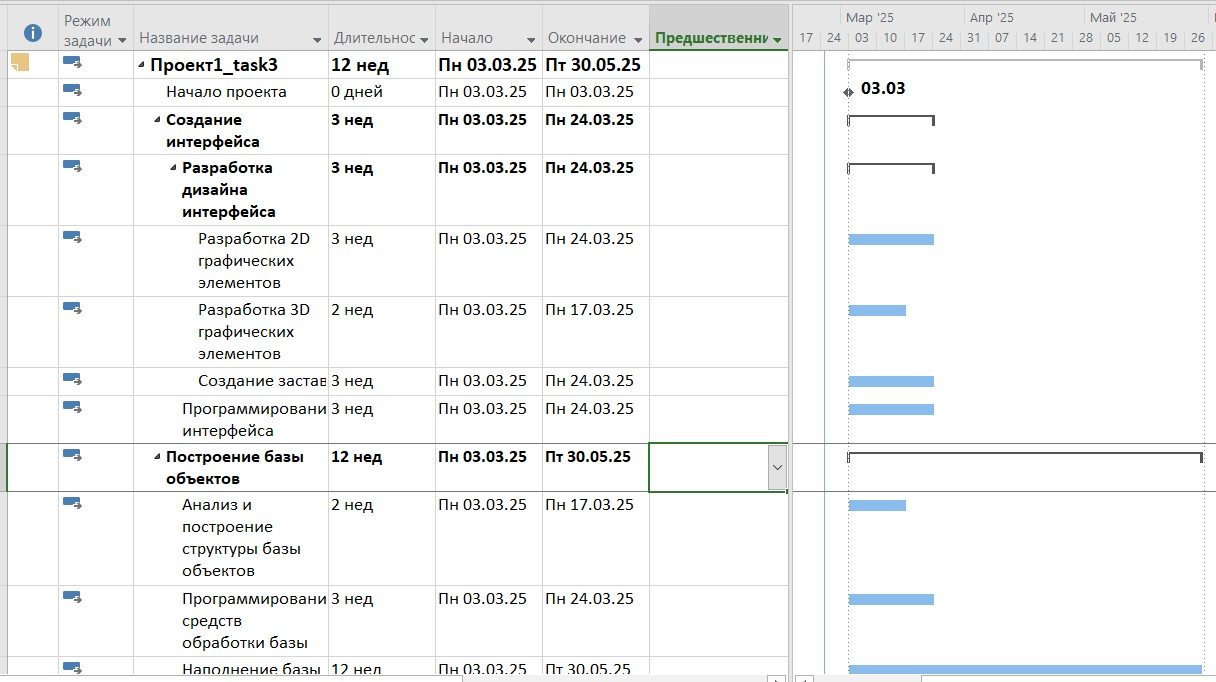
\includegraphics[width=0.9\textwidth]{img/lab1/task3/task3.jpg}
	\caption{Диаграмма Ганта после структурирования списка задач}
	\label{fig:task3}
\end{figure}

\subsection{Задание №4}

После структурирования списка задач необходимо указать связи между ними. 
Предшествующие задачи можно указать в столбце <<Предшественники>>.
По умолчанию устанавливается тип связи Окончание~---~Начало, при котором последующая задача начинается после окончания предыдущей.
В случае необходимости выбора другого типа связи необходимо дважды кликнуть по связи между задачами на диаграмме Ганта.
В появившемся модальном окне можно выбрать тип связи, а также указать время опережения/запаздывания.

Результат настройки связей между задачами приведен на рисунках~\ref{fig:task41} и~\ref{fig:task42}.

\begin{figure}[H]
	\centering
	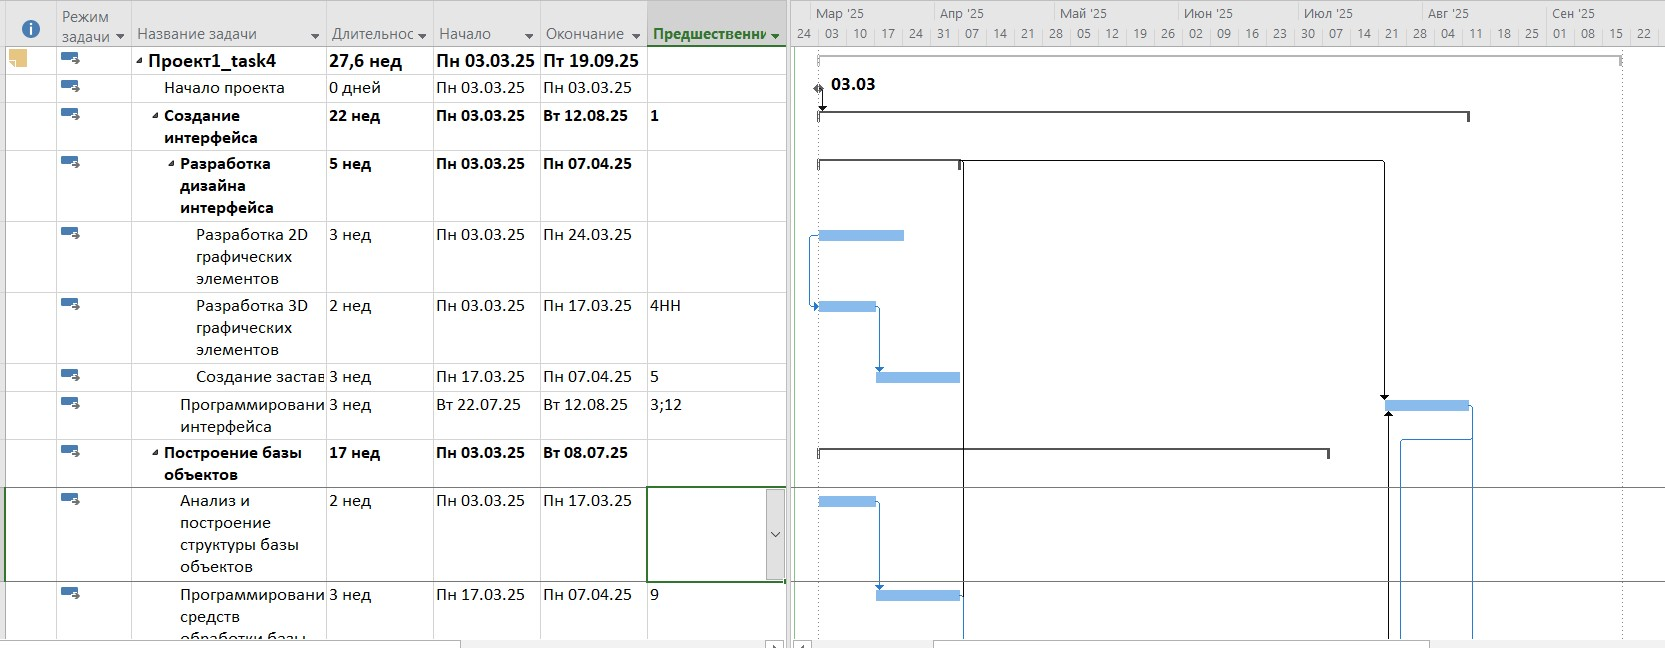
\includegraphics[width=0.9\textwidth]{img/lab1/task4/task4.jpg}
	\caption{Диаграмма Ганта с датой начала проекта}
	\label{fig:task41}
\end{figure}

\begin{figure}[H]
	\centering
	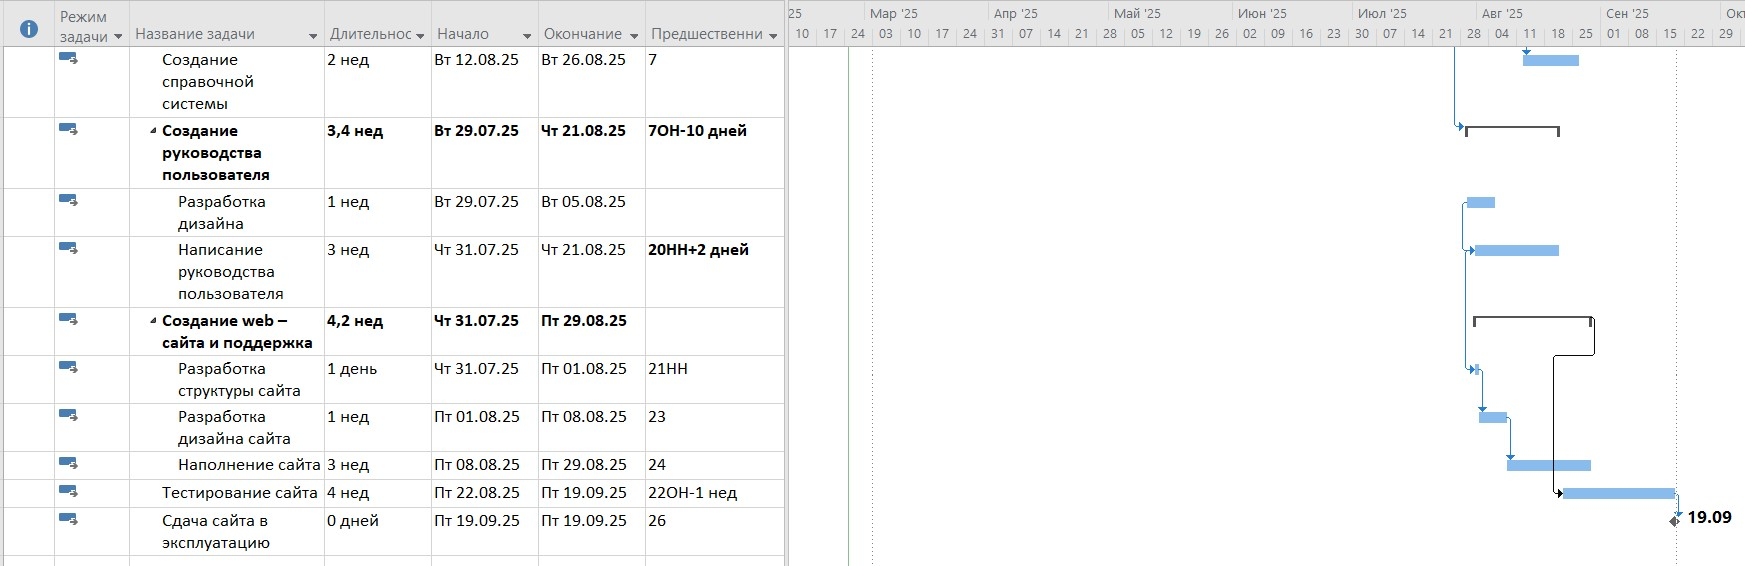
\includegraphics[width=0.9\textwidth]{img/lab1/task4/task4_1.jpg}
	\caption{Диаграмма Ганта с датой завершения проекта}
	\label{fig:task42}
\end{figure}

В результате планирования проекта было определена дата завершения проекта: 19 сентября 2025 года.
Таким образом, проект не уложился в срок 6 месяцев.

\section{Лабораторная работа №2}

\subsection{Задание для тренировки}

В лист ресурсов проекта, подготовленного в первой лабораторной работе, был добавлен трудовой ресурс <<Работник>> со стандартной ставкой 120 рублей в день и значением максимума единиц 1100\%, так как к реализации проекта привлекалось не более 11 работников.
Также был добавлен ресурс <<Оборудование>>, который арендуется по ставке 5000 рублей в неделю и на установку и наладку которого было выделено 2000 рублей.
Лист оборудования приведен на рисунке~\ref{fig:test_list}.

\begin{figure}[H]
	\centering
	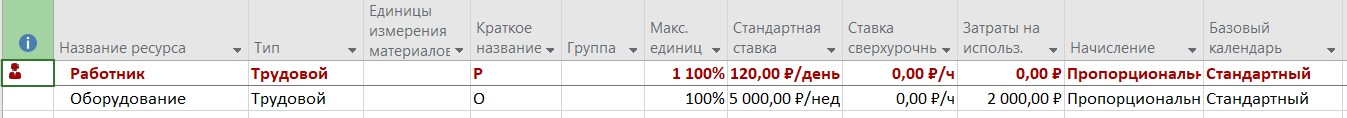
\includegraphics[width=0.9\textwidth]{img/lab2/test/equipment.jpg}
	\caption{Лист ресурсов тренировочного проекта}
	\label{fig:test_list}
\end{figure}

Так как ресурс <<Оборудование>> будет использоваться с третьего дня работы B, то необходимо установить задержку в 2 дня.
Данное действие представлено на рисунке~\ref{fig:test_delay}.

\begin{figure}[H]
	\centering
	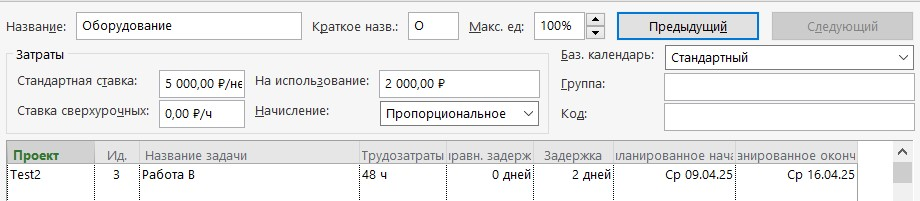
\includegraphics[width=0.9\textwidth]{img/lab2/test/delay.jpg}
	\caption{Настройка ресурса <<Оборудование>>}
	\label{fig:test_delay}
\end{figure}

В результате указания распределения ресурсов получена диаграмма Ганта, представленная на рисунке~\ref{fig:test_gant}.

\begin{figure}[H]
	\centering
	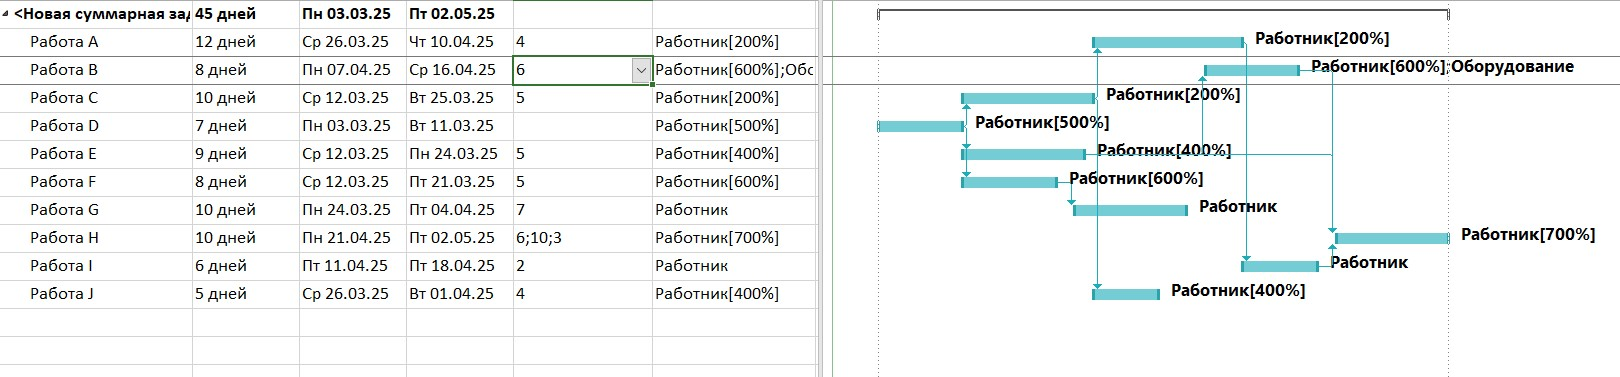
\includegraphics[width=0.9\textwidth]{img/lab2/test/add_worker.jpg}
	\caption{Диаграмма Ганта тренировочного проекта}
	\label{fig:test_gant}
\end{figure}

Полученные для ресурса <<Работник>> перегрузки демонстрируются на рисунке~\ref{fig:test_overflow}.

\begin{figure}[H]
	\centering
	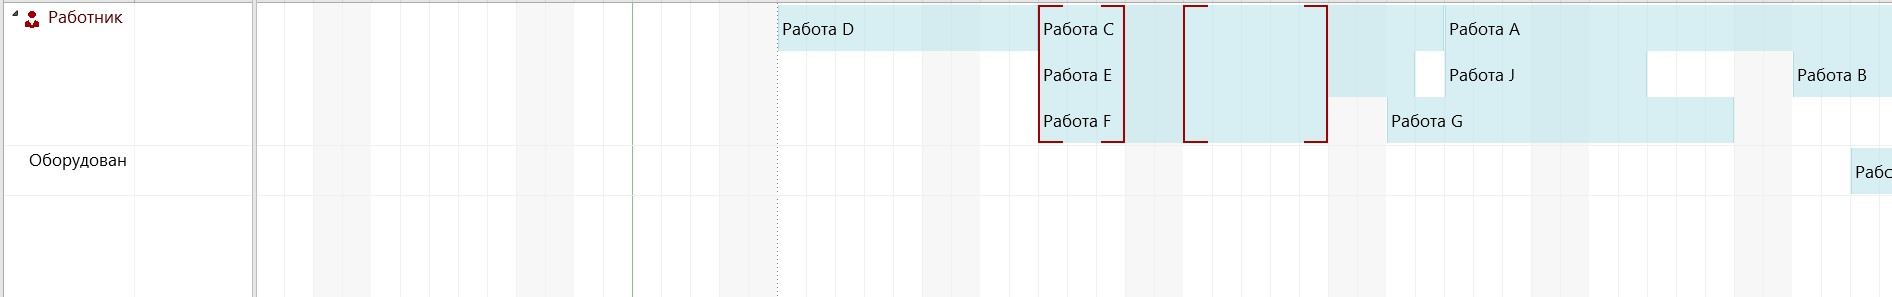
\includegraphics[width=0.9\textwidth]{img/lab2/test/overflow.jpg}
	\caption{Демонстрация перегрузки ресурса <<Работник>>}
	\label{fig:test_overflow}
\end{figure}

Перегрузка ресурса <<Работник>> возникает из-за его одновременного задействования в работах C, E и F.

На рисунке~\ref{fig:test_final} представлены затраты на проект.

\begin{figure}[H]
	\centering
	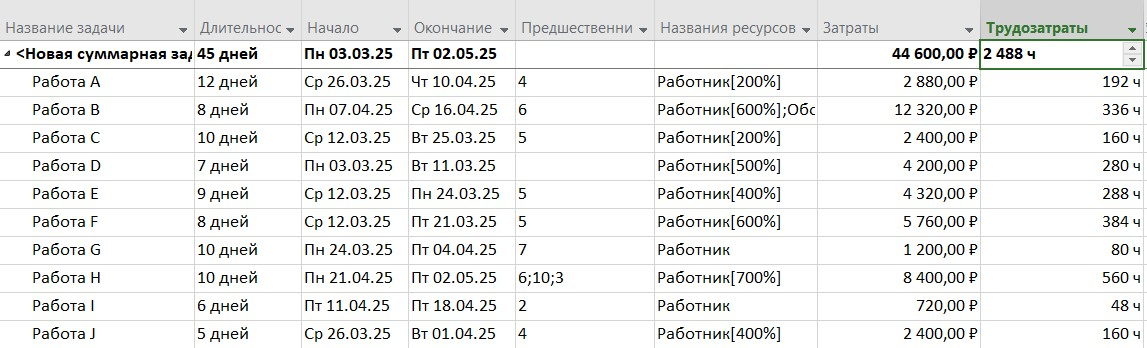
\includegraphics[width=0.9\textwidth]{img/lab2/test/final.jpg}
	\caption{Затраты на тренировочный проект}
	\label{fig:test_final}
\end{figure}

Затраты на работников составили 36600 рублей, а затраты на оборудование~---~8000 рублей.
Бюджет тренировочного проекта составил 44600 рублей.

\subsection{Задание №1}

Проект представляет собой создание карты города.
В проекте участвуют 16 разработчиков, бюджет проекта~---~50000 рублей, длительность проекта~---~6 месяцев.
Дата начала проекта~---~первый рабочий день марта текущего года.

Лист ресурсов проекта представлен на рисунке~\ref{fig:list}.

\begin{figure}[H]
	\centering
	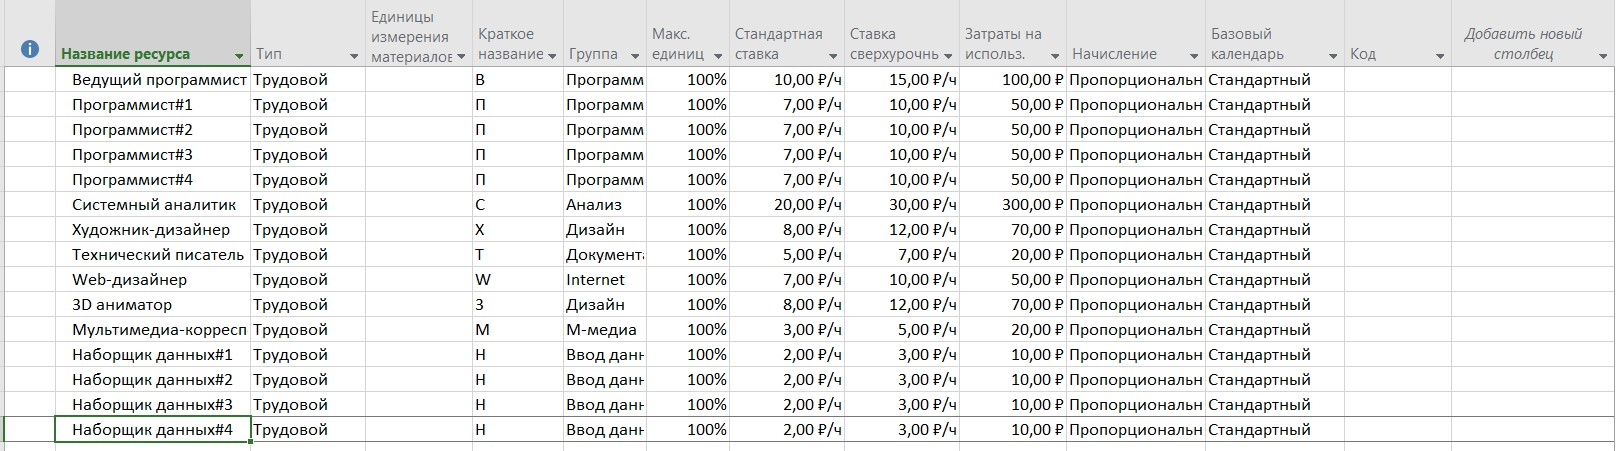
\includegraphics[width=0.9\textwidth]{img/lab2/task1/list.jpg}
	\caption{Лист ресурсов проекта}
	\label{fig:list}
\end{figure}

\subsection{Задание №2}

На рисунке~\ref{fig:gant} приведена диаграмма Ганта после назначения задачам ресурсов.

\begin{figure}[H]
	\centering
	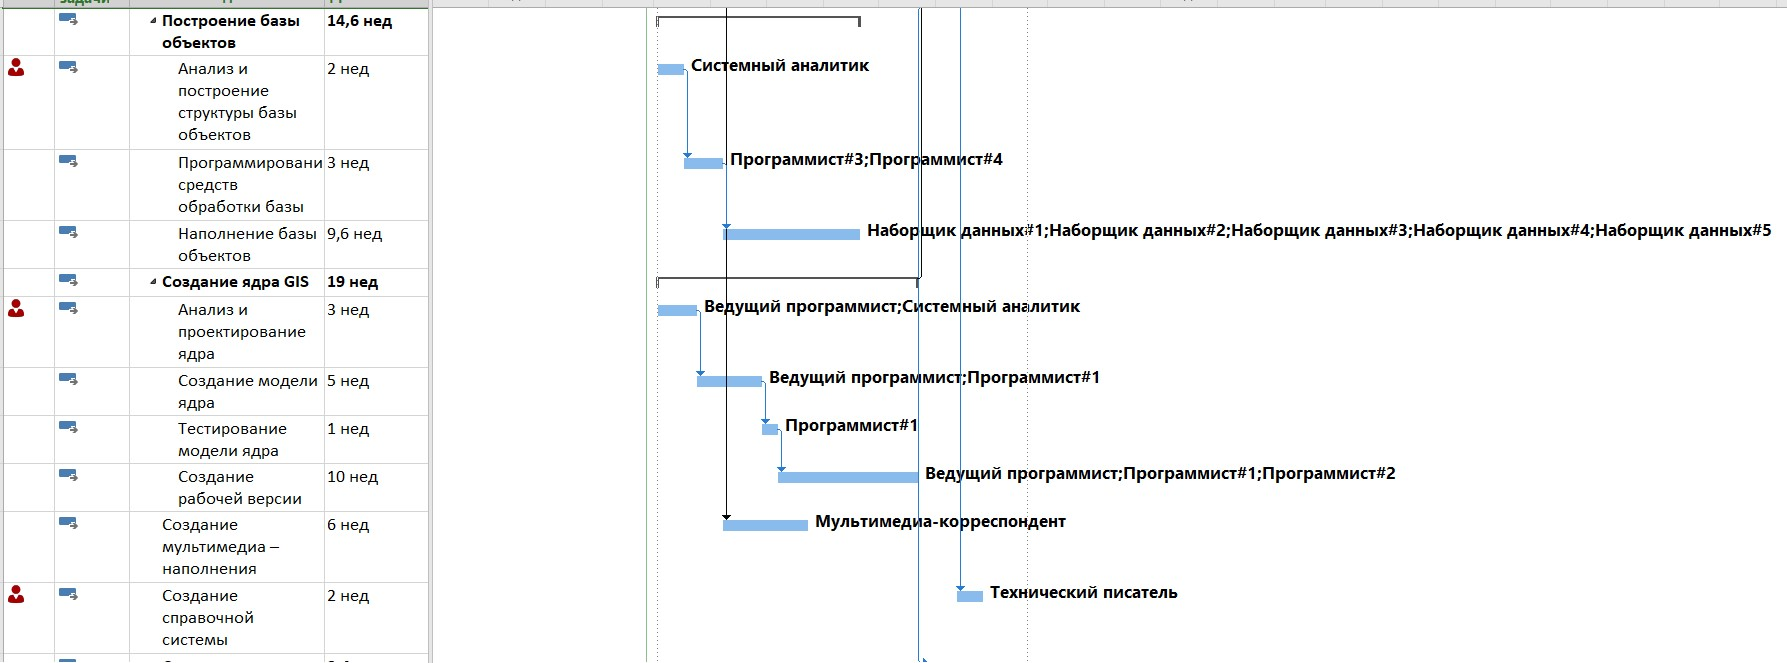
\includegraphics[width=0.9\textwidth]{img/lab2/task2/gant.jpg}
	\caption{Диаграмма Ганта после назначения ресурсов задачам проекта}
	\label{fig:gant}
\end{figure}

Как видно по диаграмме Ганта и листу ресурсов, приведенном на рисунке~\ref{fig:list_overflow}, ресурсы <<Системный аналитик>>, <<Художник-дизайнер>> и <Технический писатель>> перегружены.

\begin{figure}[H]
	\centering
	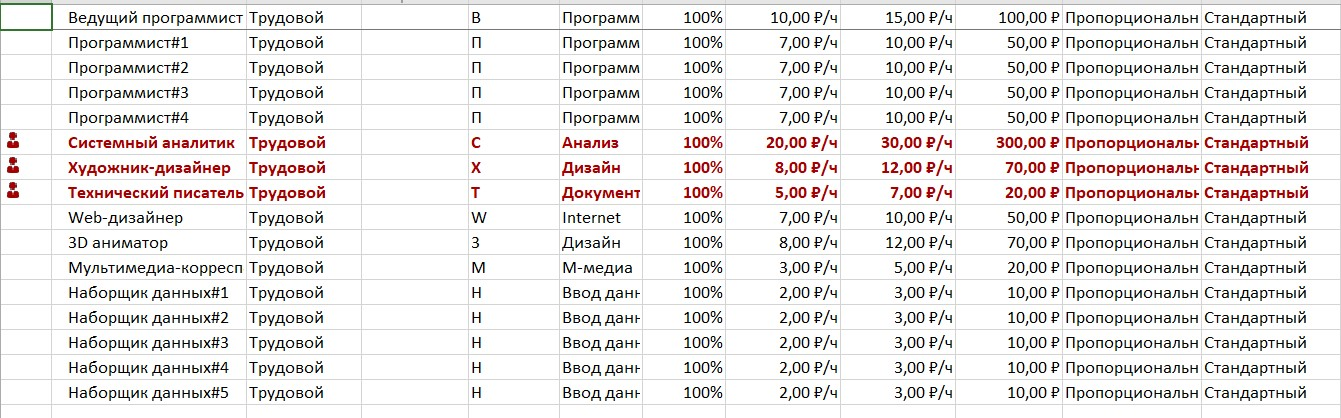
\includegraphics[width=0.9\textwidth]{img/lab2/task2/list.jpg}
	\caption{Лист ресурсов с указанием перегруженных ресурсов}
	\label{fig:list_overflow}
\end{figure}

Появление перегрузки для ресурса <<Системный аналитик>> связано с тем, что данный ресурс задействован при выполнении задач <<Анализ и построение структуры базы объектов>> и <<Анализ и проектирование ядра>>, сроки реализаций которых накладываются.

Появление перегрузки для ресурса <<Художник-дизайнер>> связано с тем, что данный ресурс задействован при выполнении задач <<Разработка дизайна руководства>> и <<Разработка дизайна сайта>>, сроки реализаций которых накладываются.

Появление перегрузки для ресурса <<Технический писатель>> связано с тем, что данный ресурс задействован при выполнении задач <<Написание руководства пользователя>> и <<Создание справочной системы>>, сроки реализаций которых накладываются.

Назначение фиксированных затрат в размере 1000 рублей на задачи 2, 8 и 12 приведено на рисунке~\ref{fig:cost}.

\begin{figure}[H]
	\centering
	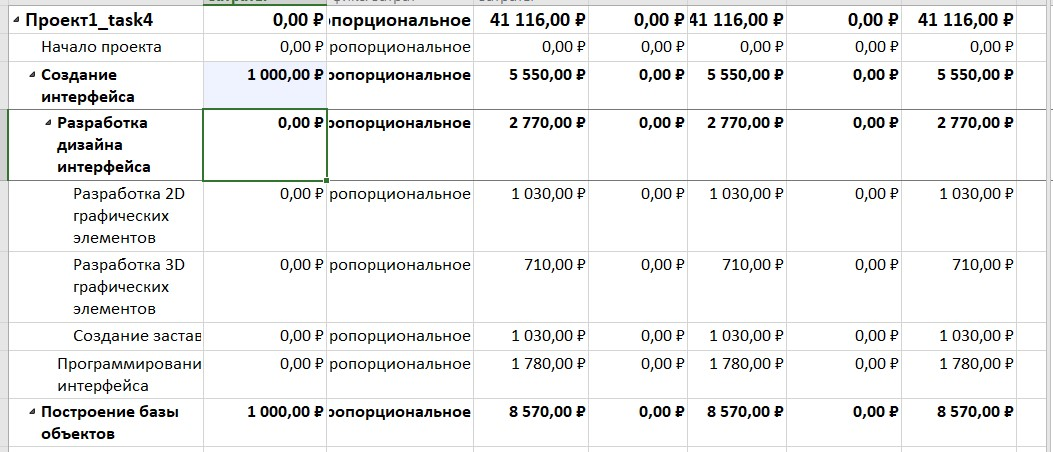
\includegraphics[width=0.9\textwidth]{img/lab2/task2/cost.jpg}
	\caption{Назначение фиксированных затрат}
	\label{fig:cost}
\end{figure}

Добавление ресурса <<Сервер>> приведено на рисунках~\ref{fig:server} и~\ref{fig:gant_server}.

\begin{figure}[H]
	\centering
	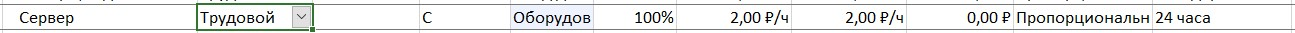
\includegraphics[width=0.9\textwidth]{img/lab2/task2/server.jpg}
	\caption{Добавление ресурса <<Сервер>> в лист ресурсов}
	\label{fig:server}
\end{figure}

\begin{figure}[H]
	\centering
	
\includegraphics[width=0.9\textwidth]{img/lab2/task2/gant_server.jpg}
	\caption{Добавление ресурса <<Сервер>> для задачи <<Построение базы объектов>>}
	\label{fig:gant_server}
\end{figure}

Сервер используется 24 часа в сутки, поэтому необходимо изменить базовый календарь на <<24 часа>>.
Так как затраты на сервер зависят от количества часов работы, он является трудовым ресурсом.

\subsection{Задание №3}

Структуризация затрат и трудозатрат по группам ресурсов и их графическое представление приведены на рисунках~\ref{fig:group}~---~\ref{fig:work_diagram}.

\begin{figure}[H]
	\centering
	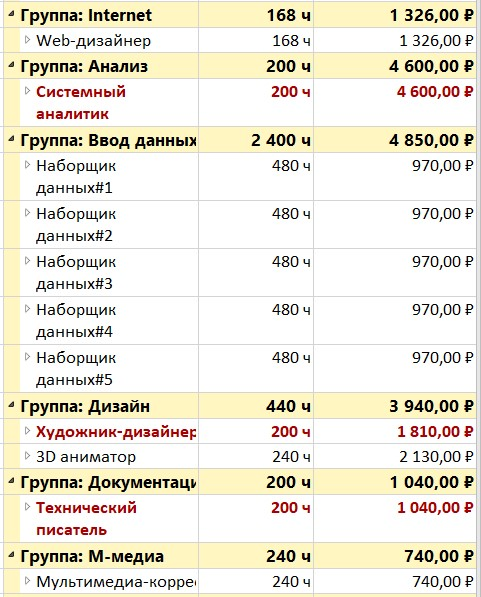
\includegraphics[width=0.9\textwidth]{img/lab2/task3/group.jpg}
	\caption{Структуризация затрат по группам ресурсов}
	\label{fig:group}
\end{figure}

\begin{figure}[H]
	\centering
	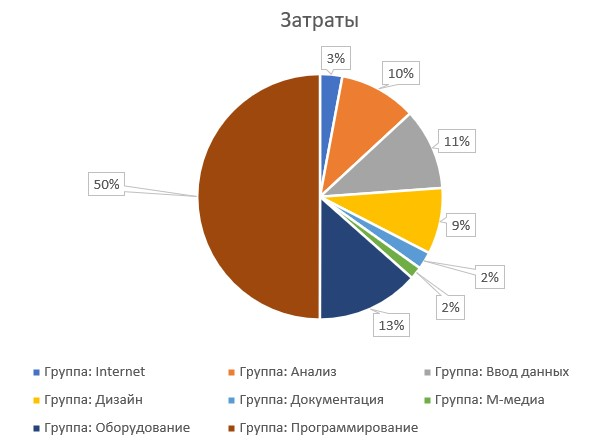
\includegraphics[width=0.9\textwidth]{img/lab2/task3/diagram.jpg}
	\caption{Графическое представление структуризации затрат по группам ресурсов}
	\label{fig:graphic_group}
\end{figure}

\begin{figure}[H]
	\centering
	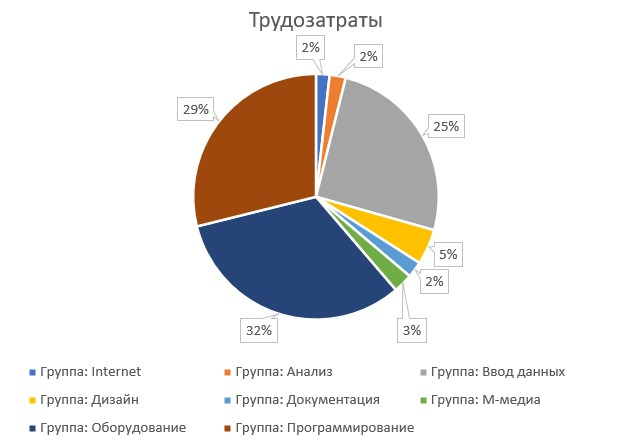
\includegraphics[width=0.9\textwidth]{img/lab2/task3/work_diagram.jpg}
	\caption{Графическое представление структуризации трудозатрат по группам ресурсов}
	\label{fig:work_diagram}
\end{figure}

Таким образом, самыми затратными ресурсами являются ресурсы группы <<Программирование>> (22580 рублей, 2720 часов) и <<Сервер>> (6102 рубля, 3051 час).
Затраты на программистов объясняются высокой квалификацией работников.
Их трудозатраты соотносятся с законом Брукса, то есть занимают 30\% времени работы.
Стоит задуматься о приобретении сервера вместо его аренды.
Группа <<Ввод данных>> (4850 рублей, 2400 часов) вносит существенный вклад в трудозатраты при сравнительно небольших затратах на ресурс.
Таким образом, можно для ускорения их работы нанять еще несколько наборщиков, так как это не сильно повлияет на затраты.
На аналитика тратится размер бюджета, несоразмерный объему работы, то есть распределение его времени работы на проекте необходимо оптимизировать.
Наименьший вклад в затраты и трудозатраты вносят ресурсы групп <<Internet>>, <<M-медиа>> и <<Документация>>.

Итоговые затраты и трудозатраты на проект приведены на рисунке~\ref{fig:final}.
\begin{figure}[H]
	\centering
	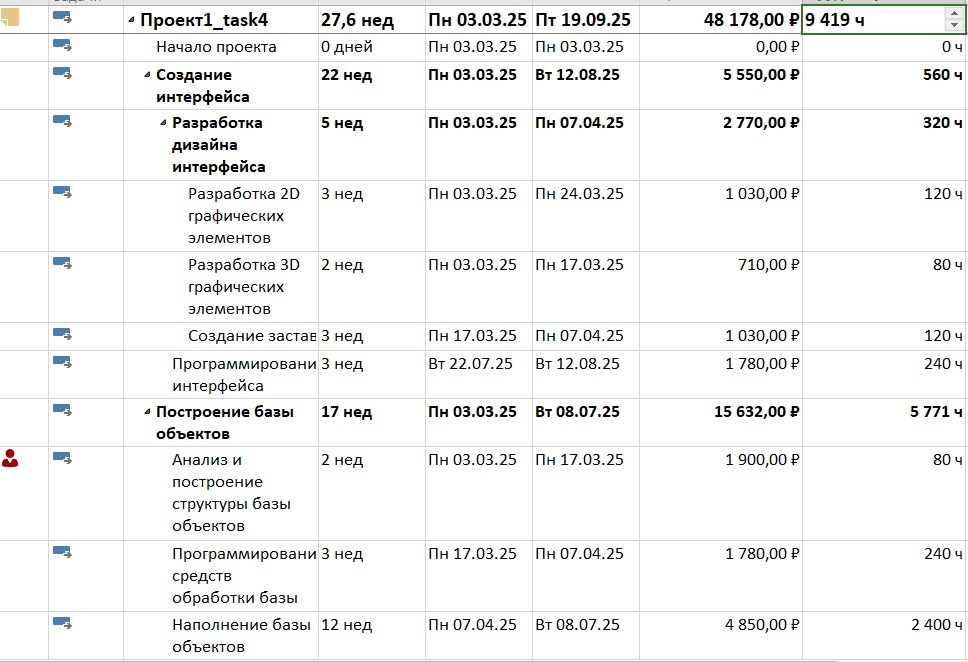
\includegraphics[width=0.9\textwidth]{img/lab2/task3/final.jpg}
	\caption{Указание затрат и трудозатрат на проект}
	\label{fig:final}
\end{figure}

Таким образом, на проект требуется 48178 рублей, что укладывается в бюджет размером 50000 рублей.

\section{Лабораторная работа №3}

\subsection{Содержание задания}
Проект представляет собой создание карты города.
В проекте участвуют 16 разработчиков, бюджет проекта~---~50000 рублей, длительность проекта~---~6 месяцев.
Дата начала проекта~---~первый рабочий день марта текущего года.

Появление перегрузки для ресурса <<Системный аналитик>> связано с тем, что данный ресурс задействован при выполнении задач <<Анализ и построение структуры базы объектов>> и <<Анализ и проектирование ядра>>, сроки реализаций которых накладываются.

Появление перегрузки для ресурса <<Художник-дизайнер>> связано с тем, что данный ресурс задействован при выполнении задач <<Разработка дизайна руководства>> и <<Разработка дизайна сайта>>, сроки реализаций которых накладываются.

Появление перегрузки для ресурса <<Технический писатель>> связано с тем, что данный ресурс задействован при выполнении задач <<Написание руководства пользователя>> и <<Создание справочной системы>>, сроки реализаций которых накладываются.

Устранить перегрузки возможно следующими способами:
\begin{itemize}[label=---]
	\item изменить календарь работы ресурса;
	\item назначить ресурс на неполный день;
	\item добавить ресурсу время задержек;
	\item применить автоматическое выравнивание.
\end{itemize}

\subsection{Задание 1}

В проекте перегружено несколько ресурсов, поэтому для устранения перегрузок необходимо использовать автоматическое выравнивание.
Параметры выравнивания представлены на рисунке~\ref{fig:screen1}.
Выравнивание должно выполняться автоматически и во всем проекте. Во избежание очистки данных предыдущего выравнивания перед новым выравниванием необходимо убрать соответствующий флажок.

\begin{figure}[H]
	\centering
	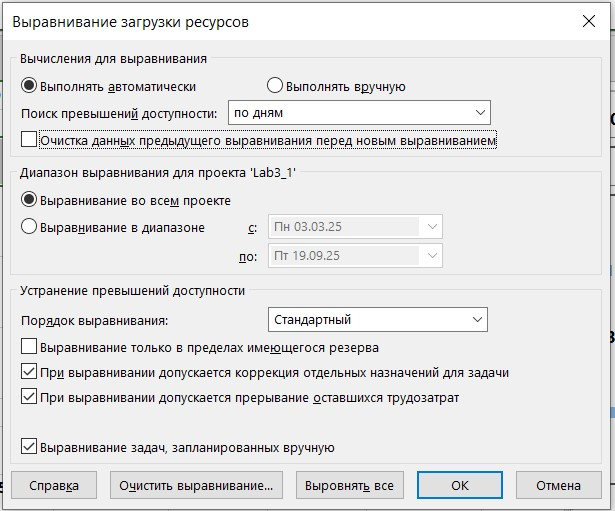
\includegraphics[width=0.9\textwidth]{img/lab3/task1/screen1.jpg}
	\caption{Параметры выравнивания}
	\label{fig:screen1}
\end{figure}

После применения автоматического выравнивания бюджет проекта сократился на 2 рубля за счет смещения вехи <<Построение базы объектов>> с 03.03 на 24.03, за счет чего работа команды не попала на предпраздничный укороченный день 07.03.
Окончание проекта сместилось с 19.09 на 23.09, а трудозатраты снизились с 9419 часов до 9418 часов.

Сведения для проекта после выравнивания отражены на рисунке~\ref{fig:screen2}.

\begin{figure}[H]
	\centering
	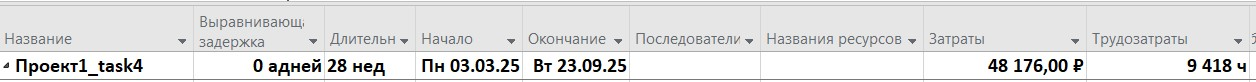
\includegraphics[width=0.9\textwidth]{img/lab3/task1/screen2.jpg}
	\caption{Сведения о проекте после выравнивания}
	\label{fig:screen2}
\end{figure}

Диаграмма Ганта после выравнивания приведена на рисунке~\ref{fig:screen3}.

\begin{figure}[H]
	\centering
	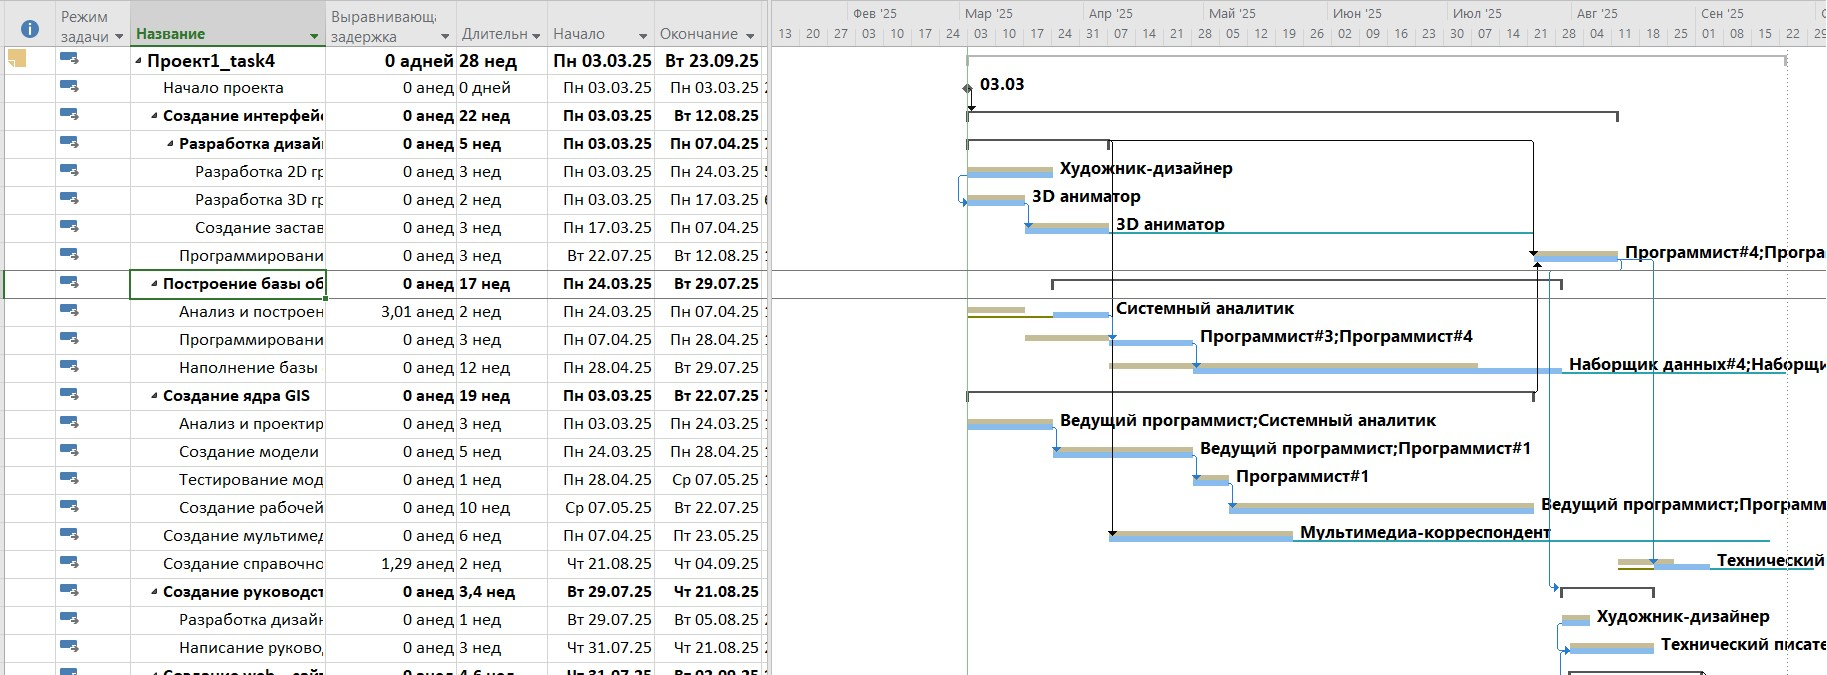
\includegraphics[width=0.9\textwidth]{img/lab3/task1/screen3.jpg}
	\caption{Диаграмма Ганта после выравнивания}
	\label{fig:screen3}
\end{figure}

Перегрузки ресурса <<Системный аналитик>> устранены за счет ввода задержки для задачи <<Анализ и построение структуры базы объектов>>.
Срок выполнения задачи до выравнивания~---~с 03.03 до 17.03, после выравнивания~---~с 24.03 до 07.04.
Задаче <<Анализ и проектирование ядра>> не могут быть добавлены задержки, так как она входит в критический путь.
Задачам критического пути нельзя добавить задержки, так как они влияют на дату окончания проекта.
Данная задержка приведена на рисунках~\ref{fig:screen4} и~\ref{fig:screen5}.

\begin{figure}[H]
	\centering
	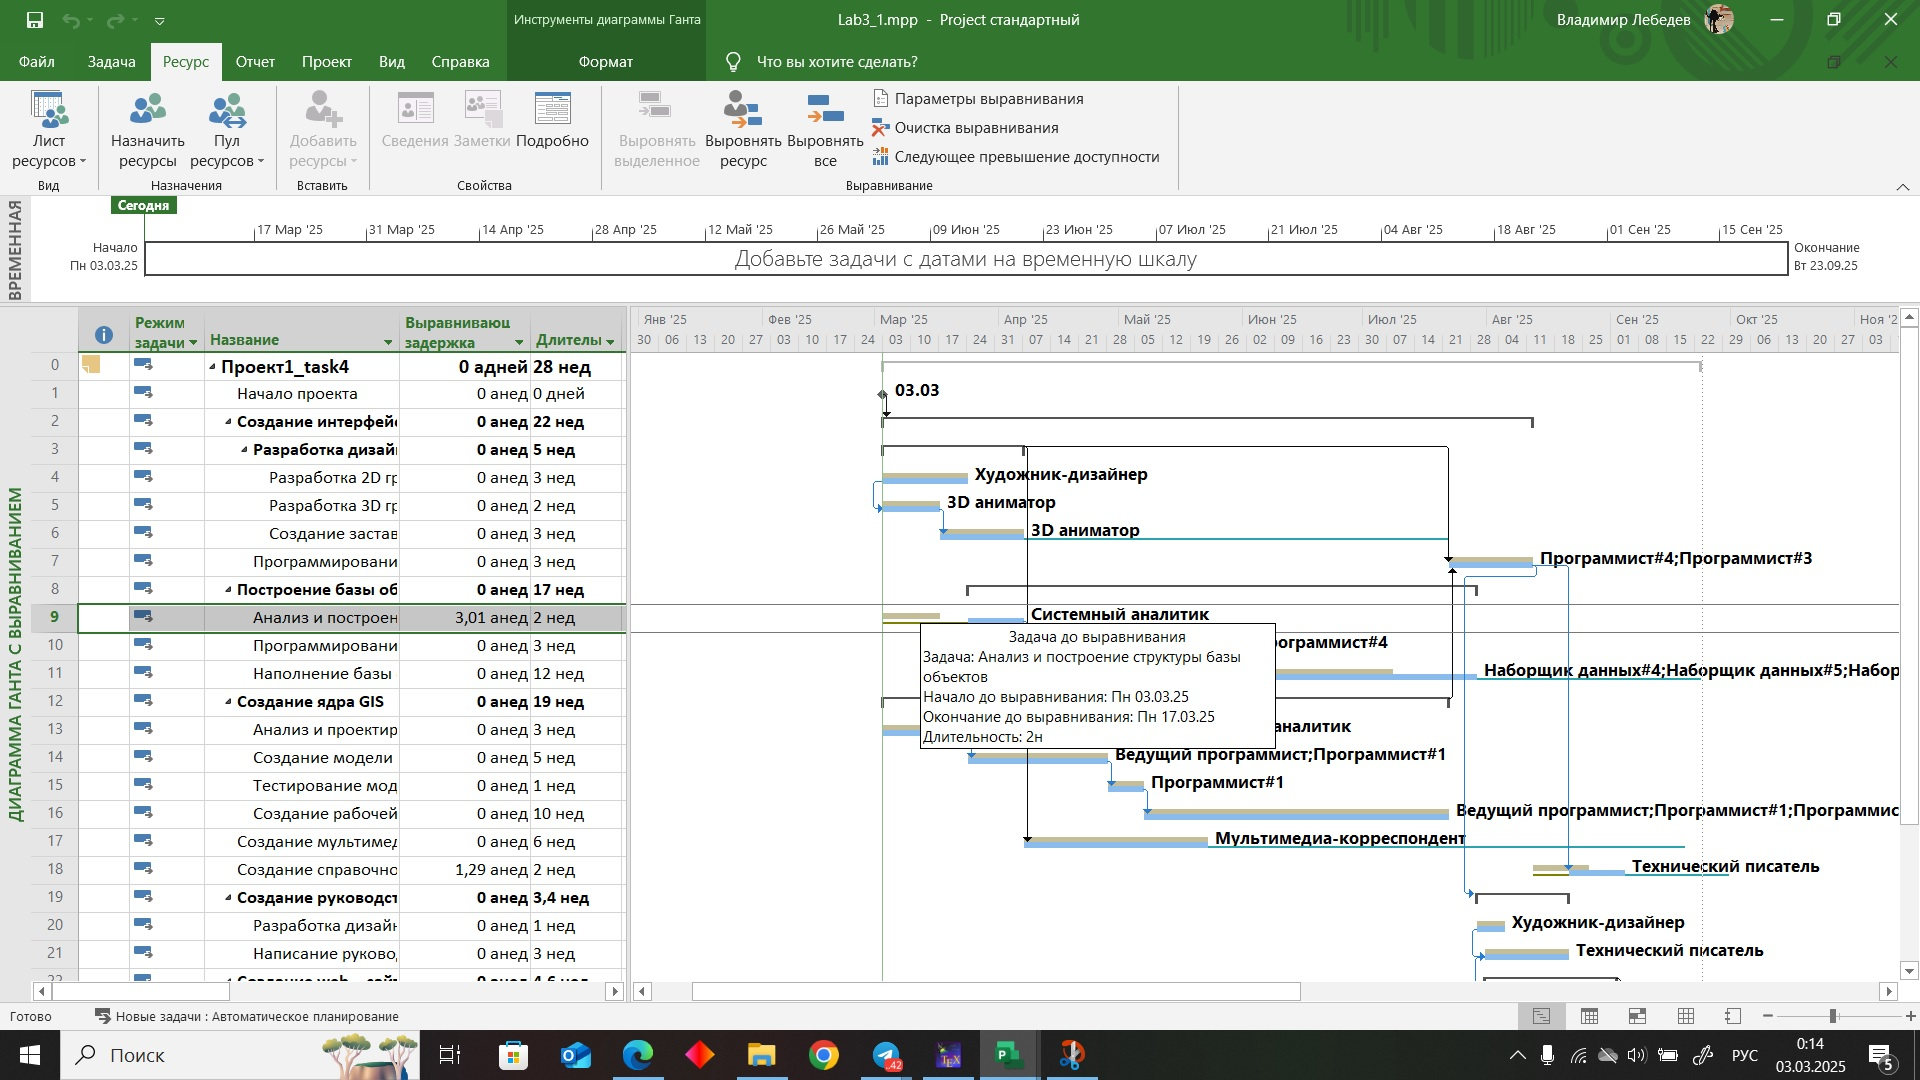
\includegraphics[width=0.9\textwidth]{img/lab3/task1/screen4.jpg}
	\caption{<<Анализ и построение структуры базы объектов>> до выравнивания}
	\label{fig:screen4}
\end{figure}

\begin{figure}[H]
	\centering
	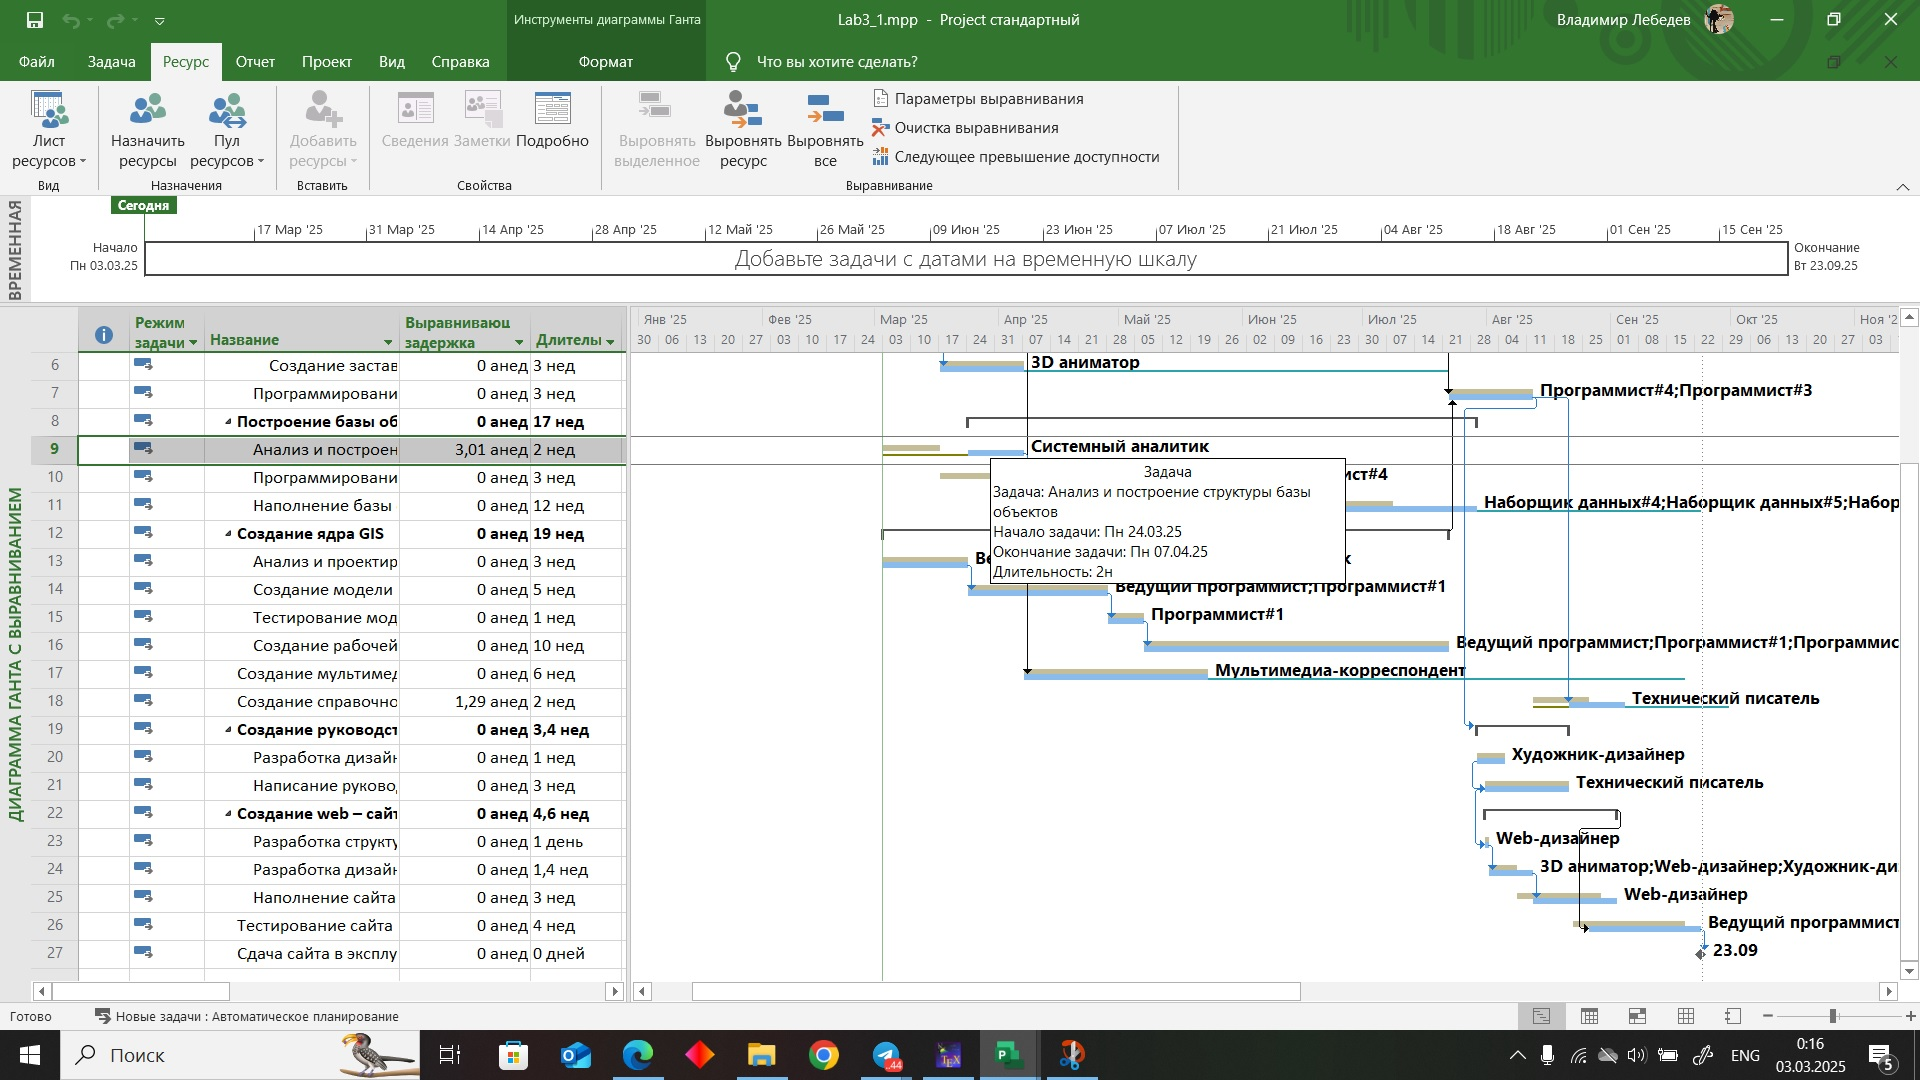
\includegraphics[width=0.9\textwidth]{img/lab3/task1/screen5.jpg}
	\caption{<<Анализ и построение структуры базы объектов>> после выравнивания}
	\label{fig:screen5}
\end{figure}

Перегрузки ресурса <<Технический писатель>> устранены за счет ввода задержки для задачи <<Создание справочной системы>>.
Срок выполнения задачи до выравнивания~---~с 12.08 до 26.08, после выравнивания~---~с 21.08 до 04.09.
Задаче <<Написание руководства пользователя>> не могут быть добавлены задержки, так как она входит в критический путь.
Данная задержка приведена на рисунках~\ref{fig:screen6} и~\ref{fig:screen7}.

\begin{figure}[H]
	\centering
	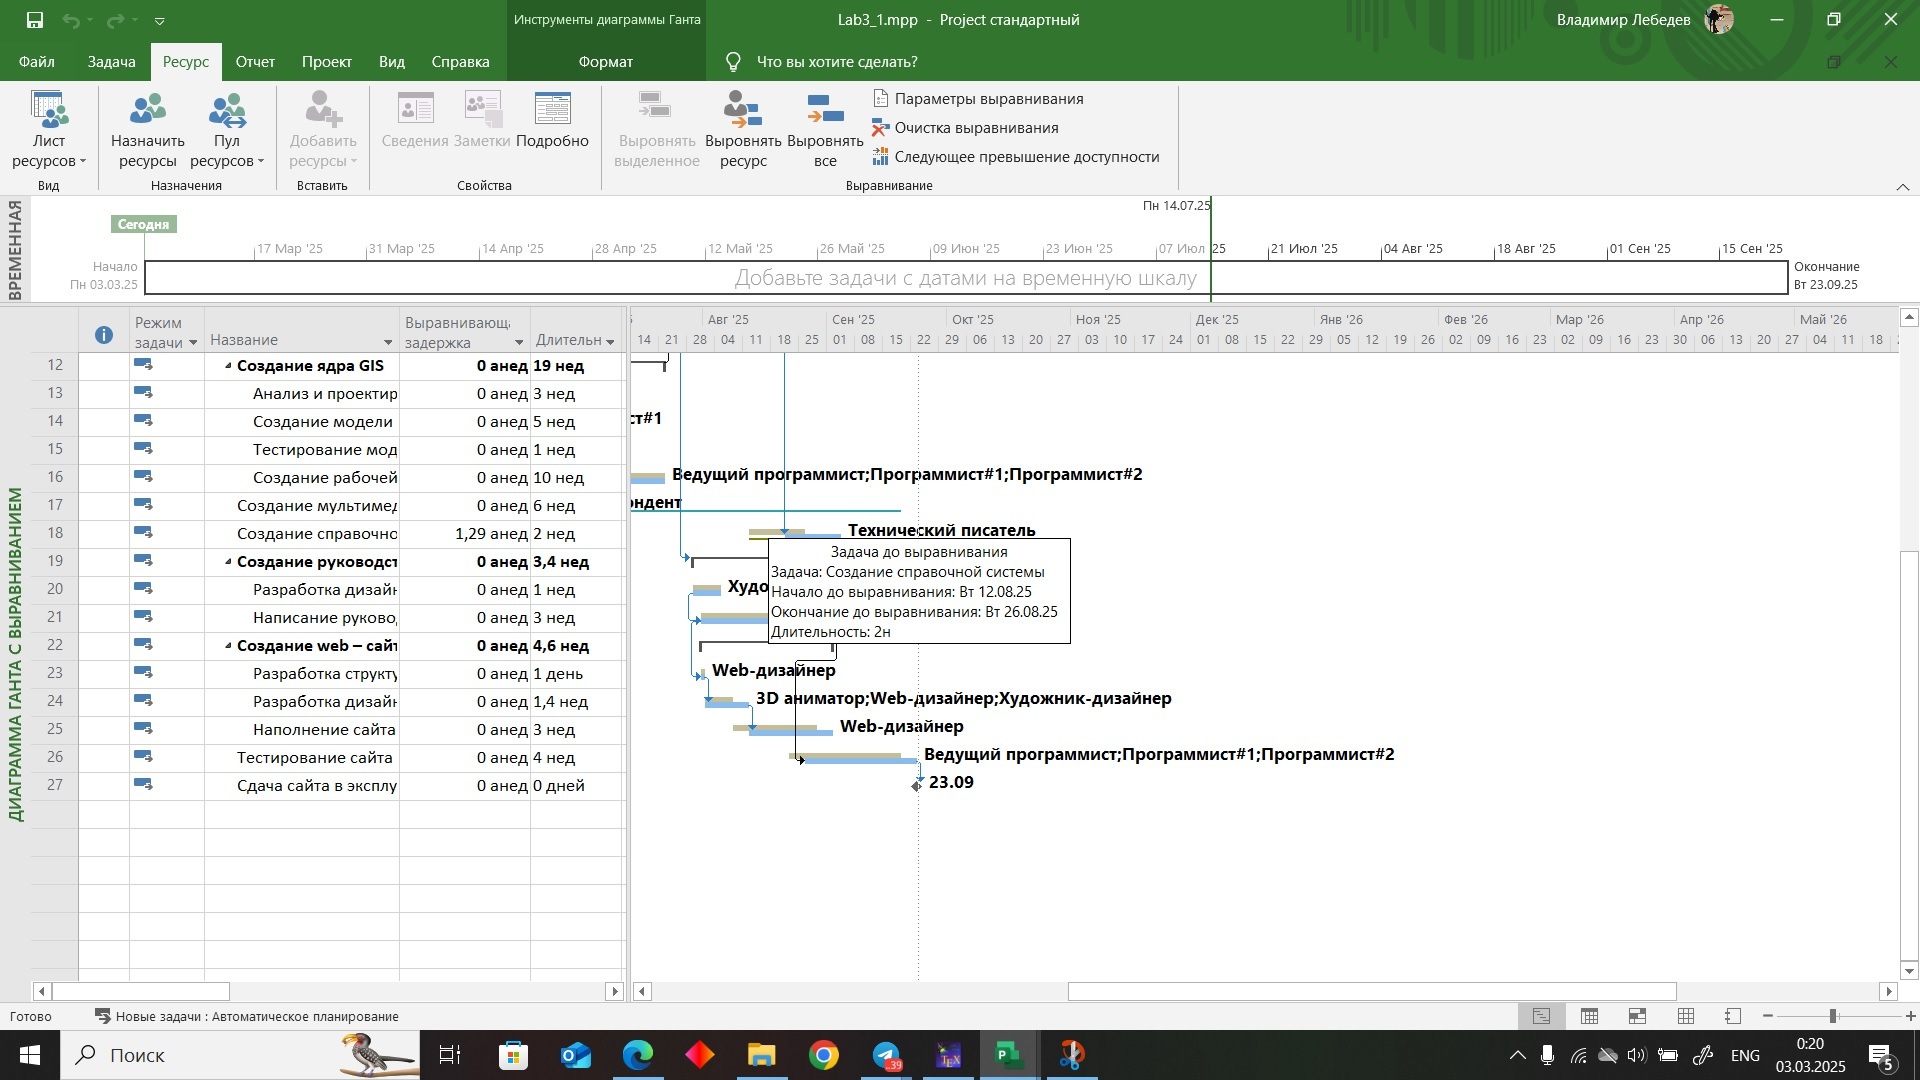
\includegraphics[width=0.9\textwidth]{img/lab3/task1/screen6.jpg}
	\caption{<<Создание справочной системы>> до выравнивания}
	\label{fig:screen6}
\end{figure}

\begin{figure}[H]
	\centering
	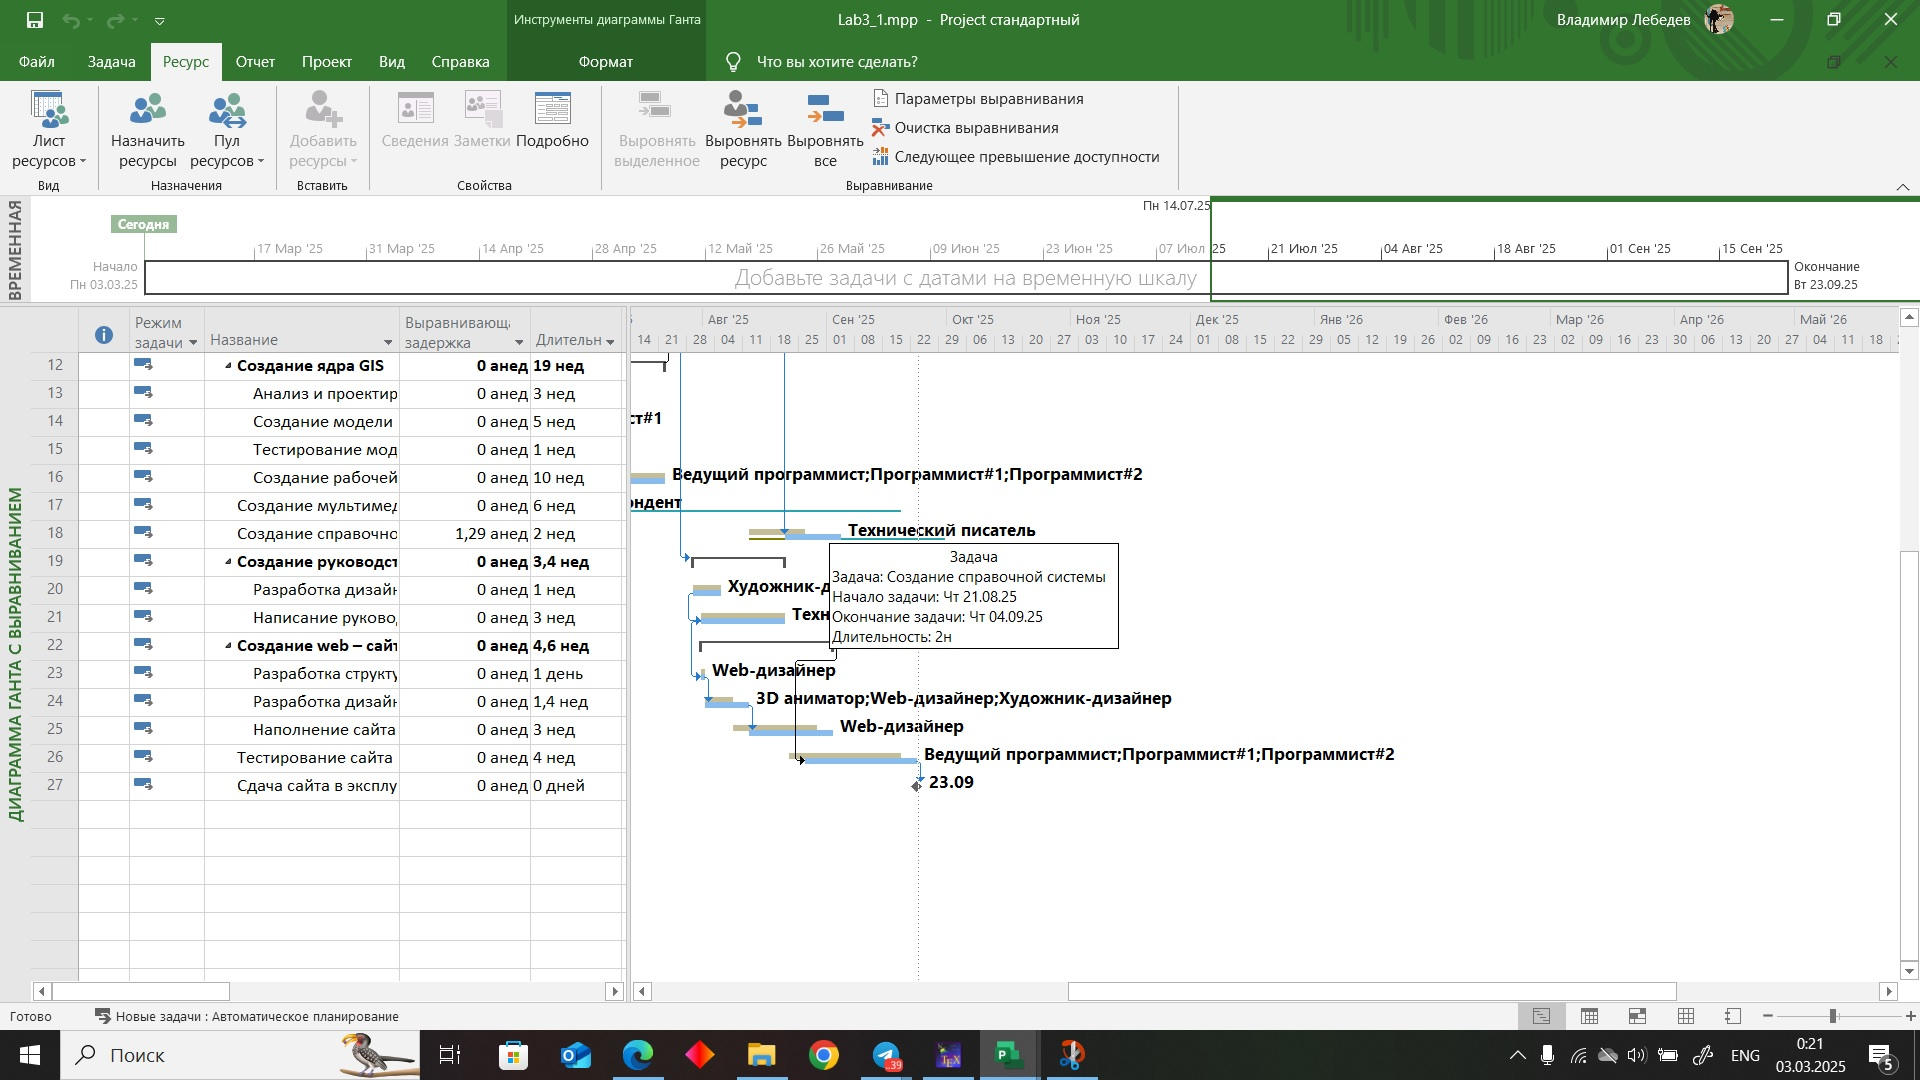
\includegraphics[width=0.9\textwidth]{img/lab3/task1/screen7.jpg}
	\caption{<<Создание справочной системы>> после выравнивания}
	\label{fig:screen7}
\end{figure}

Перегрузка ресурса <<Художник-дизайнер>> устранена путем введения задержки на 4 дня для него в рамках задачи <<Разработка дизайна сайта>>, что отражено на рисунке~\ref{fig:screen8}.
Задачи <<Разработка дизайна сайта>> и <<Разработка дизайна руководства>>, в которых участвует художник-дизайнер, входят в критический путь, из-за чего им не могут быть добавлены задержки.
Поэтому задержки добавлены для начала работы художника-дизайнера в задаче <<Разработка дизайна сайта>>, что привело к увеличению срока проекта на 4 дня.

\begin{figure}[H]
	\centering
	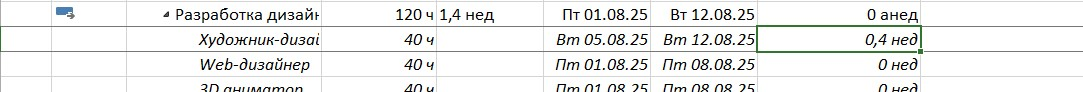
\includegraphics[width=0.9\textwidth]{img/lab3/task1/screen8.jpg}
	\caption{Задержка для ресурса <<Художник-дизайнер>> в рамках <<Разработки дизайна сайта>>}
	\label{fig:screen8}
\end{figure}

\subsection{Задание 2}

Необходимо добавить задачу <<Совещание>>, которая будет повторяться каждую среду с 10:00 до 11:00.
В совещании задействованы все специалисты кроме наборщиков и программистов №1-4.
Настройка повторяющегося события <<Совещание>> приведена на рисунке~\ref{fig:screen2_1}.

\begin{figure}[H]
	\centering
	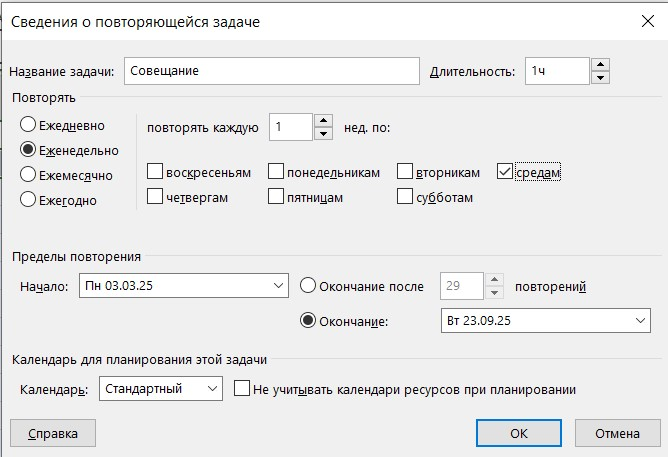
\includegraphics[width=0.9\textwidth]{img/lab3/task2/screen1.jpg}
	\caption{Настройка повторяющегося события <<Совещание>>}
	\label{fig:screen2_1}
\end{figure}

Назначение ресурсов, трудозатраты и затраты на ресурсы во время совещания, а также обновленные сроки проекта приведены на рисунке~\ref{fig:screen2_2}.
Трудозатраты на одно совещание составили 7 часов, затраты~---~691 рубль.
Суммарно на все совещания потрачено 203 часа трудозатрат и 20039 рублей.
Таким образом, окончание проекта сместилось с 19.09 на 26.09, бюджет проекта превысил заложенные 50000 рублей и составил 68219 рублей.
Перегрузка ресурсов была устранена автоматически.

\begin{figure}[H]
	\centering
	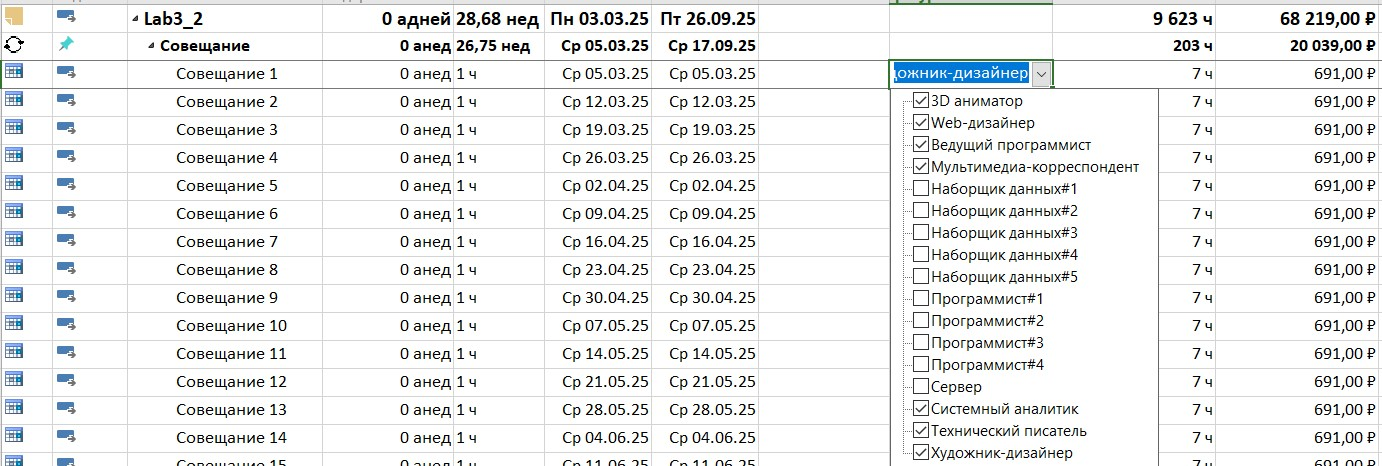
\includegraphics[width=0.9\textwidth]{img/lab3/task2/screen2.jpg}
	\caption{Изменения в проекте после добавления <<Совещания>>}
	\label{fig:screen2_2}
\end{figure}

Для всех человеческих ресурсов указаны затраты на использование, то есть дополнительные расходы, связанные с доставкой, установкой, наладкой оборудования для сотрудников, обучением персонала.
Эти затраты не следует учитывать в рамках <<Совещания>>.
Для этого необходимо ввести новую ставку, при которой затраты на использование равны нулю, что демонстрируется на рисунке~\ref{fig:screen2_3}.

\begin{figure}[H]
	\centering
	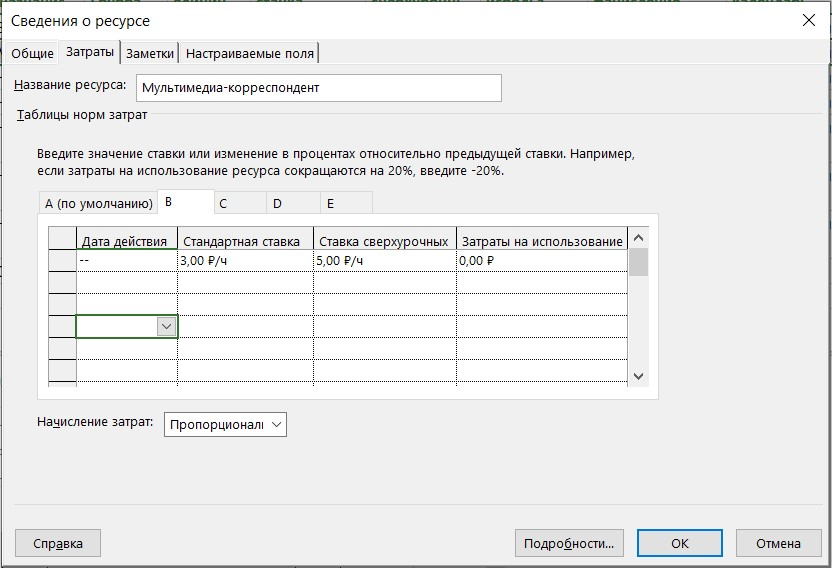
\includegraphics[width=0.9\textwidth]{img/lab3/task2/screen3.jpg}
	\caption{Добавление новой ставки для ресурса <<Мультимедиа-корреспондент>>}
	\label{fig:screen2_3}
\end{figure}

После добавления новой ставки необходимо выбрать ее для каждого ресурса, задействованного в <<Совещании>>.
Такая настройка, доступная в разделе <<Вид>> --- <<Использование задач>> --- <<Сведения о назначении>>, приведена на рисунке~\ref{fig:screen2_4}.

\begin{figure}[H]
	\centering
	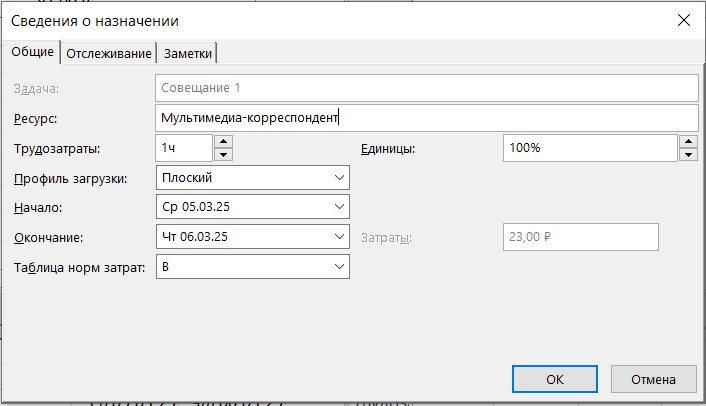
\includegraphics[width=0.9\textwidth]{img/lab3/task2/screen4.jpg}
	\caption{Смена ставки для ресурса}
	\label{fig:screen2_4}
\end{figure}

Затраты на одно совещание после смены ставки составили 61 рубль, на все совещания~---~1769 рублей, на весь проект~---~49949 рублей, что укладывается в бюджет в 50000 рублей.
Несмотря на введение новой ставки, на совещание все равно добавляются дополнительные трудозатраты, из-за чего бюджет проекта увеличился на 1769 рублей по сравнению с проектом в лабораторной работе №2, тем самым запас бюджета составляет 51 рубль.
Выравнивание выполнялось автоматически путем дробления задач.
Затраты после смены ставки приведены на рисунке~\ref{fig:screen2_5}.

\begin{figure}[H]
	\centering
	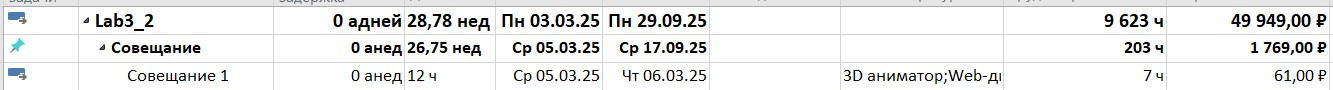
\includegraphics[width=0.9\textwidth]{img/lab3/task2/screen5.jpg}
	\caption{Затраты после смены ставки сотрудников}
	\label{fig:screen2_5}
\end{figure}

\subsection{Задание 3}

Критический путь проекта представлен на рисунке~\ref{fig:screen3_1}.

\begin{figure}[H]
	\centering
	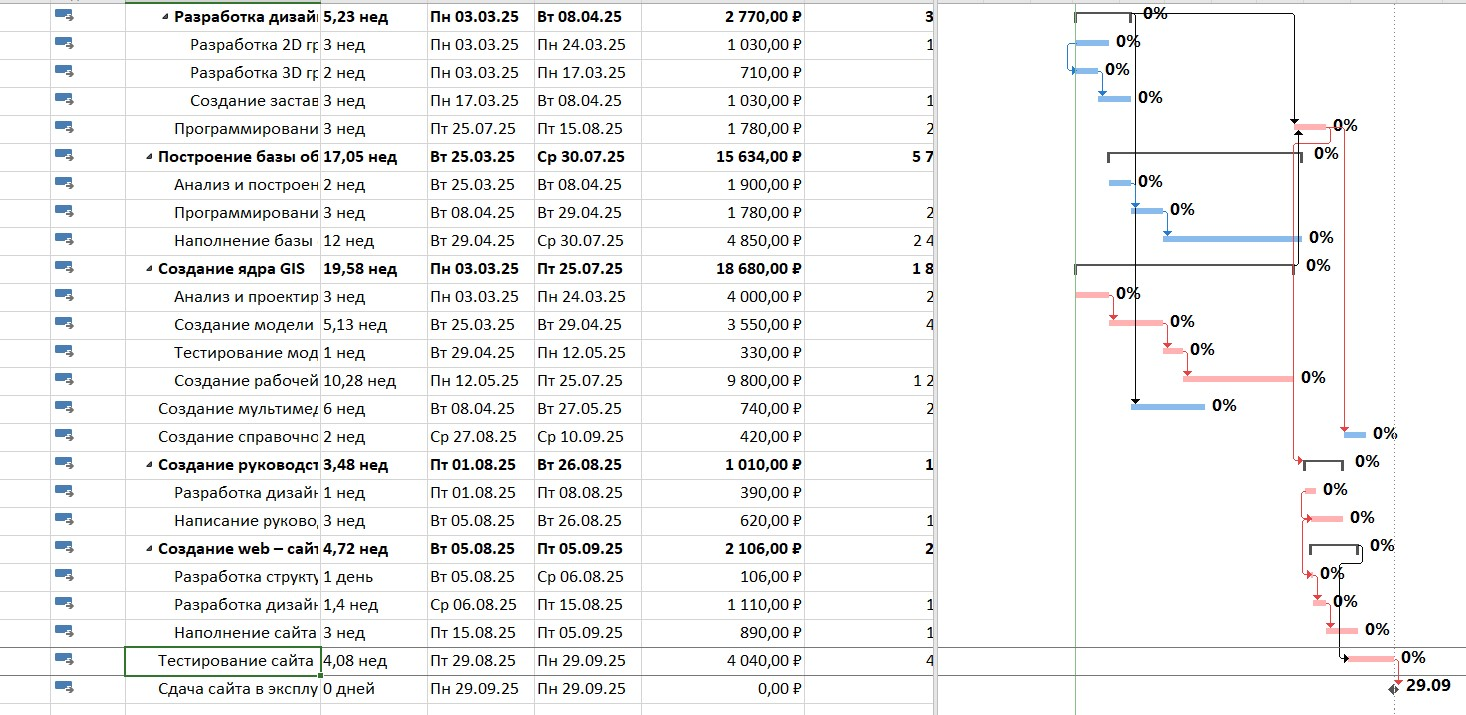
\includegraphics[width=0.9\textwidth]{img/lab3/task3/screen1.jpg}
	\caption{Критический путь проекта}
	\label{fig:screen3_1}
\end{figure}

Исходя из диаграммы Ганта с отслеживанием, критический путь состоит из задач <<Анализ и проектирование ядра>>, <<Создание модели>>, <<Тестирование модели>>, <<Создание рабочей версии ядра>>, <<Программирование интерфейса>>, <<Разработка дизайна руководства>>, <<Написание руководства пользователя>>, <<Наполнение сайта>> и <<Тестирование сайта>>.

Для оптимизации критического пути выполнены следующие действия:
\begin{itemize}[label=---]
	\item к ресурсам задачи <<Создание модели>> добавлен ресурс <<Программист №2>>;
	\item к ресурсам задачи <<Тестирование сайта>> добавлены ресурсы <<Программист №3>> и <<Программист №4>>;
	\item к ресурсам задачи <<Создание рабочей версии ядра>> добавлены ресурсы <<Программист №3>> и <<Программист №4>>.
\end{itemize}

К ресурсам задачи <<Создание модели>> не добавлены программисты №3-4, так как их добавление увеличивает затраты проекта.
Добавление ресурсов представлено на рисунке~\ref{fig:screen3_2}.
Так как задачи имеют фиксированные трудозатраты, при увеличении количества ресурсов уменьшается продолжительность задачи.
Окончание проекта сместилось на 12.08, то есть удалось сократить сроки проекта более, чем на месяц и уложиться в срок 6 месяцев.

\begin{figure}[H]
	\centering
	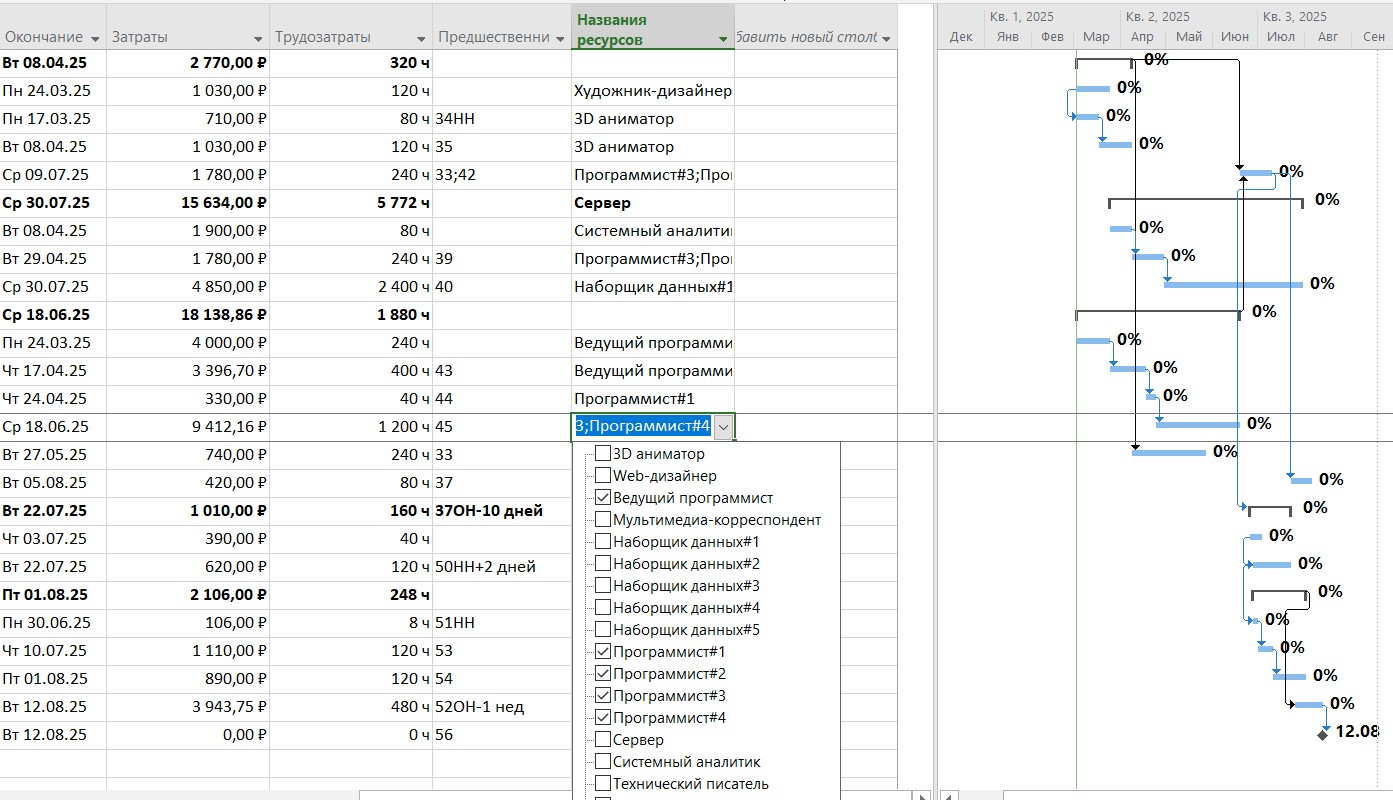
\includegraphics[width=0.9\textwidth]{img/lab3/task3/screen2.jpg}
	\caption{Добавление ресурсов}
	\label{fig:screen3_2}
\end{figure}

Так как дата окончания проекта изменилась, необходимо уменьшить число совещаний путем изменения даты окончания повторяющегося события <<Совещание>>, что продемонстрировано на рисунке~\ref{fig:screen3_3}.
Последнее совещание состоится 06.08.

\begin{figure}[H]
	\centering
	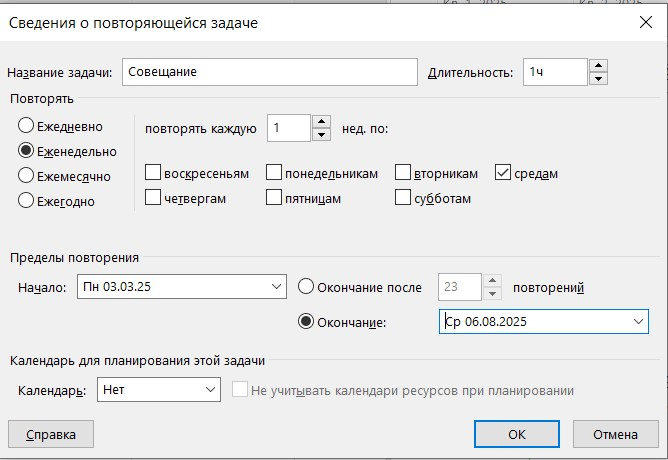
\includegraphics[width=0.9\textwidth]{img/lab3/task3/screen3.jpg}
	\caption{Изменение параметров повторяющегося события <<Совещание>>}
	\label{fig:screen3_3}
\end{figure}

Проект завершится 12.08 с затратами 48945 рублей, уложившись в срок 6 месяцев и бюджет 50000 рублей.
По сравнению с 
Информация о проекте и его статистика приведены на рисунках~\ref{fig:screen3_4} и~\ref{fig:screen3_9}.

\begin{figure}[H]
	\centering
	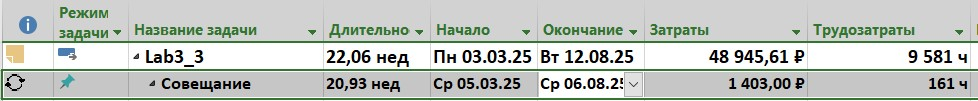
\includegraphics[width=0.9\textwidth]{img/lab3/task3/screen4.jpg}
	\caption{Информация о проекте}
	\label{fig:screen3_4}
\end{figure}

\begin{figure}[H]
	\centering
	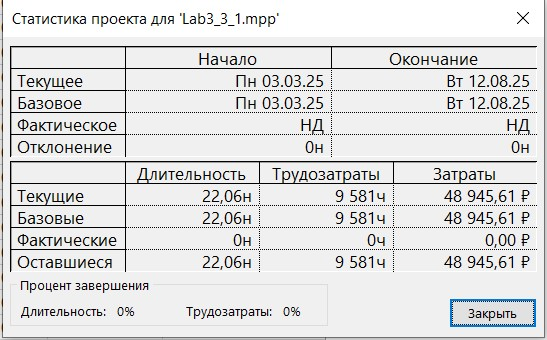
\includegraphics[width=0.9\textwidth]{img/lab3/task3/screen9.jpg}
	\caption{Статистика проекта}
	\label{fig:screen3_9}
\end{figure}

Затраты на группы ресурсов приведены на рисунке~\ref{fig:screen3_7}.

На рисунках~\ref{fig:screen3_5} и~\ref{fig:screen3_6} отображены диаграммы трудозатрат и затрат.

\begin{figure}[H]
	\centering
	
\includegraphics[width=0.9\textwidth]{img/lab3/task3/screen10.jpg}
	\caption{Затраты на группы ресурсов}
	\label{fig:screen3_7}
\end{figure}

\begin{figure}[H]
	\centering
	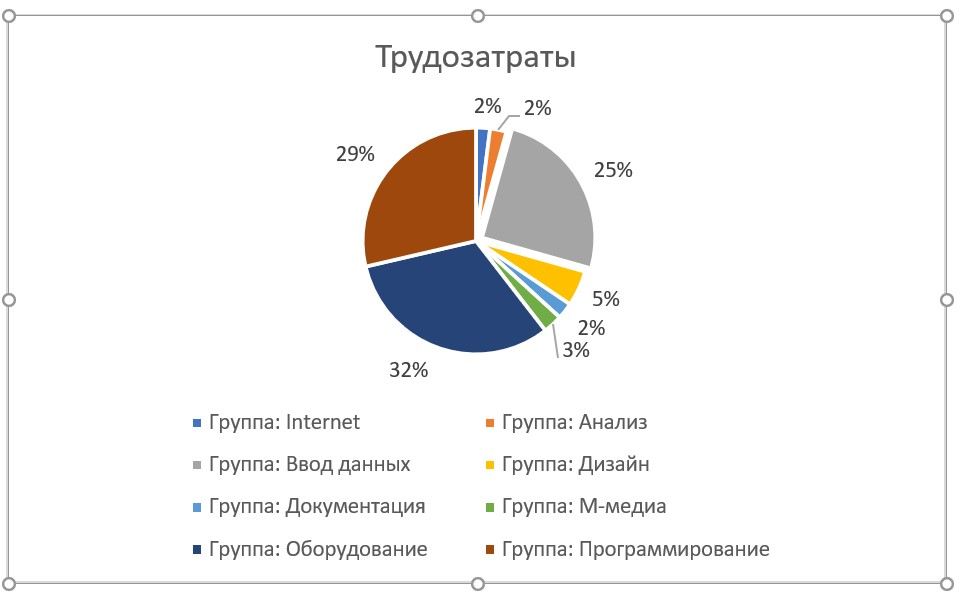
\includegraphics[width=0.9\textwidth]{img/lab3/task3/screen5.jpg}
	\caption{Диаграмма трудозатрат проекта}
	\label{fig:screen3_5}
\end{figure}

\begin{figure}[H]
	\centering
	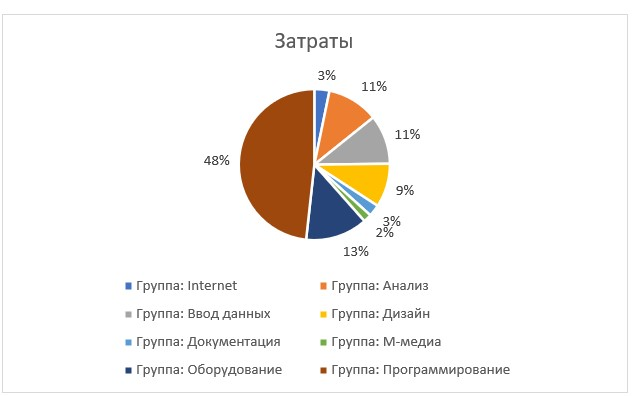
\includegraphics[width=0.9\textwidth]{img/lab3/task3/screen6.jpg}
	\caption{Диаграмма затрат проекта}
	\label{fig:screen3_6}
\end{figure}

По сравнению с лабораторной работой №2 затраты на программистов снизились на 2\% (с 50\% до 48\%), а на аналитика и технического писателя увеличились на 1\% (с 10\% до 11\% и с 2\% до 3\% соответственно).
Затраты на сервер выросли на 2 рубля и составили 6104 рубля.
Затраты на программистов снизились с 22580 рублей до 22172 рублей.
Затраты повысились из-за фиксированных трудозатрат, необходимых на выполнение задач и добавления 23 совещаний по 1 часу.
Проценты распределения трудозатрат не изменились, так как тип задач~---~фиксированные трудозатраты.

Затраты на программистов объясняются высокой квалификацией работников.
Их трудозатраты соотносятся с законом Брукса, то есть занимают 30\% времени работы.
Стоит задуматься о приобретении сервера вместо его аренды.
Группа <<Ввод данных>> (4850 рублей, 2400 часов) вносит существенный вклад в трудозатраты при сравнительно небольших затратах на ресурс.
Таким образом, можно для ускорения их работы нанять еще несколько наборщиков, так как это не сильно повлияет на затраты.
На аналитика тратится размер бюджета, несоразмерный объему работы, то есть распределение его времени работы на проекте необходимо оптимизировать.
Наименьший вклад в затраты и трудозатраты вносят ресурсы групп <<Internet>>, <<M-медиа>> и <<Документация>>.

Сохранение базового плана проекта продемонстрировано на рисунке~\ref{fig:screen3_8}.

\begin{figure}[H]
	\centering
	
\includegraphics[width=0.9\textwidth]{img/lab3/task3/screen8.jpg}
	\caption{Сохранение базового плана проекта}
	\label{fig:screen3_8}
\end{figure}

\section{Лабораторная работа №4}

\subsection{Внесение фактических данных}

Дата начала проекта в соответствии с базовым планом~---~03.03.2025, дата окончания проекта~---12.08.2025.
Затраты на проект в соответствии с базовым планом составляют 48945 рублей. 

По заданию дата отчета~---~11.05.2025.
Установка даты отчета показана на рисунке~\ref{fig:4_screen1}.

\begin{figure}[H]
	\centering
	
\includegraphics[width=0.9\textwidth]{img/lab4/screen1_report.jpg}
	\caption{Дата отчета}
	\label{fig:4_screen1}
\end{figure}

По заданию с 10 марта на 2 недели заболел 3D-аниматор.
В это время его обязанности выполнял художник-дизайнер, совмещая их со своими работами по проекту из расчета 60\% доступности по своим задачам и 40\% по задачам 3D-аниматора.
В этот период зарплата художника-дизайнера увеличилась на 10\%.

Необходимо установить 0\% занятости 3D-аниматора в период с 10.03 по 23.03 в связи с его болезнью, что продемонстрировано на рисунке~\ref{fig:4_screen2}. 

\begin{figure}[H]
	\centering
	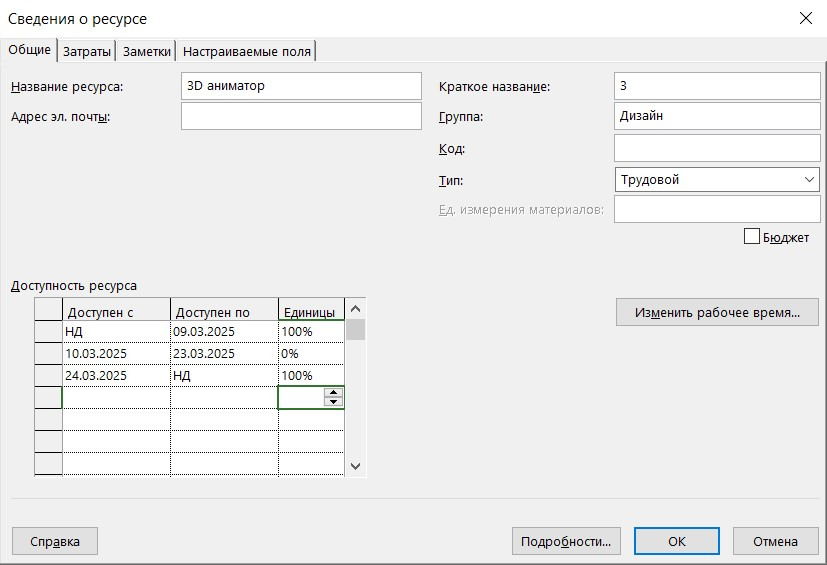
\includegraphics[width=0.9\textwidth]{img/lab4/screen2.jpg}
	\caption{Отражение информации о болезни 3D-аниматора}
	\label{fig:4_screen2}
\end{figure}

Также на этот период зарплата художника-дизайнера выросла на 10\%, обновленная стандартная ставка составила 8.8 рублей в час, а ставка сверхурочных~---13.2 рубля в час, что отражено на рисунке~\ref{fig:4_screen3}.
Занятость по собственным задачам у художника-аниматора составила 60\%, что отражено на рисунке~\ref{fig:4_screen4}.

\begin{figure}[H]
	\centering
	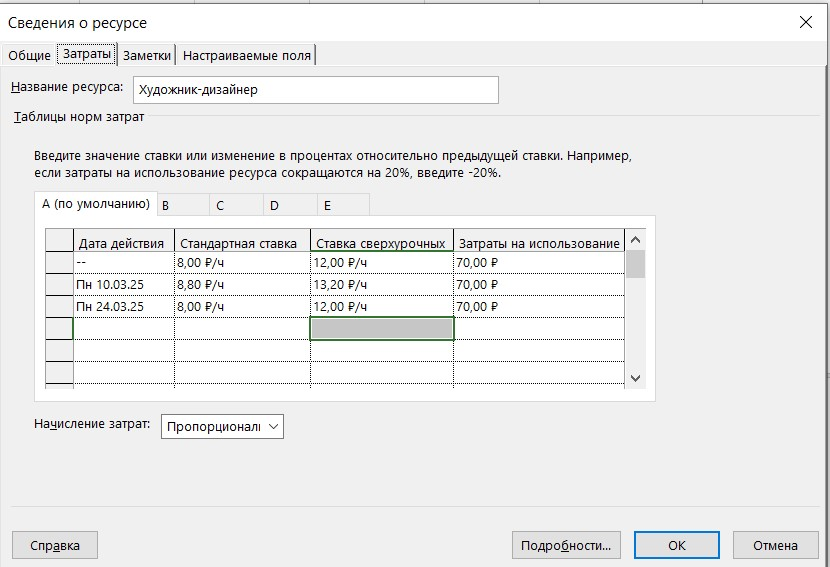
\includegraphics[width=0.9\textwidth]{img/lab4/screen3.jpg}
	\caption{Изменение ставки художника-дизайнера на период болезни 3D-аниматора}
	\label{fig:4_screen3}
\end{figure}

\begin{figure}[H]
	\centering
	\includegraphics[width=0.9\textwidth]{img/lab4/screen4.jpg}
	\caption{Обновление нагрузки по собственным задачам художника-дизайнера}
	\label{fig:4_screen4}
\end{figure}

Задача <<Разработка 3D графических элементов>> 3D-аниматора, длящаяся с 03.03 по 17.03, попадает в период болезни 3D-аниматора, поэтому необходимо назначить на нее художника-дизайнера с 40\% занятости, что приведено на рисунке~\ref{fig:screen32}.

\begin{figure}[H]
	\centering
	\includegraphics[width=0.9\textwidth]{img/lab4/screen32.jpg}
	\caption{Назначение художника-дизайнера на задачу 3D-аниматора}
	\label{fig:screen32}
\end{figure}

В представлении <<Использование задач>> необходимо указать сроки назначения художника-аналитика на задачу.
Из-за частичной загрузки художника-дизайнера дата окончания задачи <<Разработка 2D графических элементов>> смещается с 24.03 на 01.04, а дата окончания задачи <<Разработка 3D графических элементов>>~---~с 17.03 на 27.03.

Возникает перегрузка ресурса <<Художник-дизайнер>> из-за того, что на этот период его нагрузка ограничена 60\%, что составляет 4.8 часа в день, а задача <<Разработка 3D графических элементов>> вносит дополнительную нагрузку в 0.19 часа в день параллельно с задачей художника-аниматора <<Разработка 2D графических элементов>>.
Однако суммарная загрузка художника-аниматора за рабочий день не превышает 8 часов, что отражено на рисунке~\ref{fig:4_screen6}, поэтому данным предупреждением от Microsoft Project можно пренебречь.

\begin{figure}[H]
	\centering
	\includegraphics[width=0.9\textwidth]{img/lab4/screen6.jpg}
	\caption{Дневная загрузка художника-аниматора в период болезни 3D-дизайнера}
	\label{fig:4_screen6}
\end{figure}

Также на период болезни 3D-аниматора необходимо убрать его с совещаний.
Тем самым трудозатраты на совещания 12.03 и 19.03 сокращаются с 7 часов до 6 часов, что показано на рисунке~\ref{fig:4_screen7}.

\begin{figure}[H]
	\centering
	\includegraphics[width=0.9\textwidth]{img/lab4/screen7.jpg}
	\caption{Сокращение трудозатрат на совещания 12.03 и 19.03}
	\label{fig:4_screen7}
\end{figure}

Так как художник-дизайнер присутствует на совещании, необходимо указать для него занятость 100\% вместо установленных 60\% на этот период, что показано на рисунке~\ref{fig:4_screen8}.

\begin{figure}[H]
	\centering
	\includegraphics[width=0.9\textwidth]{img/lab4/screen8.jpg}
	\caption{Задание нагрузки художника-дизайнера на совещании}
	\label{fig:4_screen8}
\end{figure}

По заданию задача <<Разработка 3D графических элементов>> фактически завершилась 19.03, что необходимо отразить в разделе <<По графику>> --- <<Обновление задач>>, как показано на рисунке~\ref{fig:screen9}.

\begin{figure}[H]
	\centering
	\includegraphics[width=0.9\textwidth]{img/lab4/screen9.jpg}
	\caption{Задание фактической даты окончания задачи <<Разработка 3D графических элементов>>}
	\label{fig:screen9}
\end{figure}

Обновленные даты занятости ресурсов для задачи <<Разработка 3D графических элементов>> приведены на рисунке~\ref{fig:screen10}.

\begin{figure}[H]
	\centering
	\includegraphics[width=0.9\textwidth]{img/lab4/screen10.jpg}
	\caption{Даты занятости ресурсов для задачи <<Разработка 3D графических элементов>>}
	\label{fig:screen10}
\end{figure}

Таким образом, дата начала задачи <<Создание заставки>> 3D-аниматора смещается на 24.03, однако так как по базовому плану она должна начинаться 17.03, на нее также необходимо назначить художника-дизайнера на 20.03 и 21.03, после чего с 24.03 ей будет заниматься выздоровевший 3D-аниматор.
Назначение художника-дизайнера на задачу <<Создание заставки>> приведено на рисунках~\ref{fig:screen33} и~\ref{fig:screen10_1}.

\begin{figure}[H]
	\centering
	\includegraphics[width=0.9\textwidth]{img/lab4/screen33.jpg}
	\caption{Назначение художника-дизайнера на задачу <<Создание заставки>>}
	\label{fig:screen33}
\end{figure}

\begin{figure}[H]
	\centering
	\includegraphics[width=0.9\textwidth]{img/lab4/screen10_1.jpg}
	\caption{Задание сроков занятости художника-дизайнера на задаче <<Создание заставки>>}
	\label{fig:screen10_1}
\end{figure}

Для художника-дизайнера возникают перегрузки, вызванные тем, что на этот период его нагрузка ограничена 60\%, что составляет 4.8 часа в день, а задача <<Создание заставки>> вносит дополнительную нагрузку в 3.01 часа в день, что суммарно не превосходит 8 часов в день, следовательно этой перегрузкой в Microsoft Project можно пренебречь.

\begin{figure}[H]
	\centering
	\includegraphics[width=0.9\textwidth]{img/lab4/screen16.jpg}
	\caption{Демонстрация занятости художника-дизайнера в период работы над задачей <<Создание заставки>>}
	\label{fig:screen16}
\end{figure}

По заданию с 01.04 совещания стали проводиться раз в две недели и на них должны присутствовать только ведущий программист, аналитик, мультимедиа-корреспондент, веб-дизайнер и технический писатель.

Ограничение старых совещаний показано на рисунке~\ref{fig:screen11}.

\begin{figure}[H]
	\centering
	\includegraphics[width=0.9\textwidth]{img/lab4/screen11.jpg}
	\caption{Ограничение старых совещаний}
	\label{fig:screen11}
\end{figure}

Создание повторяющегося раз в две недели события новых совещаний, назначения им ресурсов и задания этим ресурсам ставки, не учитывающей затраты на использование, показаны на рисунках~\ref{fig:screen13}~---~\ref{fig:screen15}.

\begin{figure}[H]
	\centering
	\includegraphics[width=0.9\textwidth]{img/lab4/screen13.jpg}
	\caption{Создание повторяющегося события новых совещаний}
	\label{fig:screen13}
\end{figure}

\begin{figure}[H]
	\centering
	\includegraphics[width=0.9\textwidth]{img/lab4/screen14.jpg}
	\caption{Назначение ресурсов на новые совещания}
	\label{fig:screen14}
\end{figure}

\begin{figure}[H]
	\centering
	\includegraphics[width=0.9\textwidth]{img/lab4/screen15.jpg}
	\caption{Задание ставки без затрат на использование во время совещания}
	\label{fig:screen15}
\end{figure}

Полученные в итоге совещания приведены на рисунке~\ref{fig:screen12}.

\begin{figure}[H]
	\centering
	\includegraphics[width=0.9\textwidth]{img/lab4/screen12.jpg}
	\caption{Итоги по изменениям совещаний}
	\label{fig:screen12}
\end{figure}

Трудозатраты снизились с 159 часов до 76 часов, затраты~---~с 1387 рублей до 678 рублей, то есть трудозатраты и затраты на совещания удалось сократить более чем в 2 раза путем их проведения раз в 2 недели и участия в них более узкого круга специалистов с 1 апреля.

По заданию задачи <<Анализ и построение структуры базы объектов>> и <<Программирование средств обработки базы объектов>> фактически длились на 20\% дольше, то есть 2.4 и 3.6 недель вместо 2 и 3 недель соответственно.
Обновление фактической длительности задач представлено на рисунках~\ref{fig:screen17} и~\ref{fig:screen18}.

\begin{figure}[H]
	\centering
	\includegraphics[width=0.9\textwidth]{img/lab4/screen17.jpg}
	\caption{Обновление фактической длительности задачи <<Анализ и построение структуры базы объектов>>}
	\label{fig:screen17}
\end{figure}

\begin{figure}[H]
	\centering
	\includegraphics[width=0.9\textwidth]{img/lab4/screen18.jpg}
	\caption{Обновление фактической длительности задачи <<Программирование средств обработки базы объектов>>}
	\label{fig:screen18}
\end{figure}

При устранении перегрузок, возникших для программистов №3 и №4 в задаче <<Создание рабочей версии ядра>> из-за задержки по срокам задачи  <<Программирование средств обработки базы объектов>>, задача <<Создание рабочей версии ядра>> становится дольше на 1 день и завершается 19.06, что отражено на рисунках~\ref{fig:screen19} и~\ref{fig:screen20}.

\begin{figure}[H]
	\centering
	\includegraphics[width=0.9\textwidth]{img/lab4/screen19.jpg}
	\caption{Возникновение перегрузки в задаче <<Создание рабочей версии ядра>>}
	\label{fig:screen19}
\end{figure}

\begin{figure}[H]
	\centering
	\includegraphics[width=0.9\textwidth]{img/lab4/screen20.jpg}
	\caption{Смещение даты окончания задачи <<Создание рабочей версии ядра>> после устранения перегрузок}
	\label{fig:screen20}
\end{figure}

Для остальных задач можно выставить, что они завершились вовремя, что достигается в разделе <<Проект>> --- <<Обновить задачу>>, как показано на рисунке~\ref{fig:screen34}.

\begin{figure}[H]
	\centering
	\includegraphics[width=0.9\textwidth]{img/lab4/screen34.jpg}
	\caption{Фиксирование сроков завершения задач в отчетный период}
	\label{fig:screen34}
\end{figure}

По заданию с 01.04 было решено отказаться от аренды сервера, для чего был куплен собственный сервер за 4000 рублей.

Добавление нового сервера, являющегося материальным ресурсом, показано на рисунках~\ref{fig:screen21} и~\ref{fig:screen22}, отказ от аренды сервера~---~на рисунке~\ref{fig:screen23}.

\begin{figure}[H]
	\centering
	\includegraphics[width=0.9\textwidth]{img/lab4/screen21.jpg}
	\caption{Добавление нового сервера в качестве материального ресурса}
	\label{fig:screen21}
\end{figure}

\begin{figure}[H]
	\centering
	\includegraphics[width=0.9\textwidth]{img/lab4/screen22.jpg}
	\caption{Цена купленного сервера}
	\label{fig:screen22}
\end{figure}

\begin{figure}[H]
	\centering
	\includegraphics[width=0.9\textwidth]{img/lab4/screen23.jpg}
	\caption{Отмена аренды сервера}
	\label{fig:screen23}
\end{figure}

Необходимо добавить новый сервер в ресурсы вехи <<Построение базы объектов>>, а также указать дату окончания использования арендованного сервера (31 марта), что продемонстрировано на рисунках~\ref{fig:screen24} и~\ref{fig:screen25}.

\begin{figure}[H]
	\centering
	\includegraphics[width=0.9\textwidth]{img/lab4/screen24.jpg}
	\caption{Добавление нового сервера в вехе <<Построение базы объектов>>}
	\label{fig:screen24}
\end{figure}

\begin{figure}[H]
	\centering
	\includegraphics[width=0.9\textwidth]{img/lab4/screen25.jpg}
	\caption{Изменение сроков аренды сервера}
	\label{fig:screen25}
\end{figure}

Трудозатраты на использование арендованного сервера сократились с 3052 часов до 153 часов, затраты на аренду снизились с 6104 рублей до 306 рублей. 
Тем самым суммарные затраты на два сервера равны 4306 рублей, что почти в 1.5 раза меньше затрат на аренду сервера.

\subsection{Сравнение плановых и фактических показателей проекта}

Для сравнения плановых плановых и фактических показателей проекта были добавлены столбцы <<Базовое начало>>, <<Базовое окончание>>, <<Отклонение начала>>, <<Отклонение окончания>>, <<Базовые затраты>>, <<Отклонение по стоимости>>, <<Базовые трудозатраты>>, <<Отклонение по трудозатратам>>.
Резуьтаты приведены на рисунках~\ref{fig:screen26}~---~\ref{fig:screen28}.

\begin{figure}[H]
	\centering
	\includegraphics[width=0.9\textwidth]{img/lab4/screen26.jpg}
	\caption{Сравнение плановых и фактических показателей, часть 1}
	\label{fig:screen26}
\end{figure}

\begin{figure}[H]
	\centering
	\includegraphics[width=0.9\textwidth]{img/lab4/screen27.jpg}
	\caption{Сравнение плановых и фактических показателей, часть 2}
	\label{fig:screen27}
\end{figure}

\begin{figure}[H]
	\centering
	\includegraphics[width=0.9\textwidth]{img/lab4/screen28.jpg}
	\caption{Сравнение плановых и фактических показателей, часть 3}
	\label{fig:screen28}
\end{figure}

На рисунке~\ref{fig:screen35} приведена диаграмма Ганта с отслеживанием процентов завершения задач.

\begin{figure}[H]
	\centering
	\includegraphics[width=0.9\textwidth]{img/lab4/screen35.jpg}
	\caption{Диаграмма Ганта с отслеживанием процентов завершения}
	\label{fig:screen35}
\end{figure}

На совещания потрачено меньше на 85 трудочасов, 725 рублей, чем было запланировано.

Создание интерфейса закончилось на день позже запланированного, что не является критичным.
На 11.05 (дата отчета) завершен 71\% работы в рамках этой вехи.
На него было потрачено на 530 рублей и 75 трудочасов меньше запланированного, основной вклад в это внесла веха разработки дизайна интерфейсов.
В ней на 224 и 333 рубля меньше, на 30.4 и 45.2 трудочаса меньше запланированного понадобилось на задачи разработки 2D и 3D графических элементов.
Также эта веха была завершена на 0.85 недели позже запланированного.

Веха <<Построение базы объектов>> заканчивается позже на неделю из-за задержки начала задачи <<Наполнение базы объектов>>.
На 11.05 завершено 33\%, что с учетом прогнозируемой задержки на неделю не является критичным, так как наборщики данных не задействованы больше ни в одной задаче.
На оценки отклонения трудозатрат и затрат для вехи может влиять неполная завершенность задач этой вехи.

Веха <<Создание ядра GIS>> задерживается на 0.07 недели, что не является критичным.
Завершение создания мультимедиа-наполнения на 1.42 недели позже не критично, так как от этой задачи ни одна другая не зависит.

Весь проект завершается 13.08, на день позже плана, что однако с запасом укладывается в сроки проекта.
По оценкам из отчета бюджет снизился на 3000 рублей.

\subsection{Линия прогресса}

Для отображения линии прогресса необходимо выполнить действия в разделе <<Формат>> --- <<Сетка>> --- <<Линии хода выполнения>>, показанные на рисунке~\ref{fig:screen29}.
Необходимо отобразить линию прогресса на дату отчета о состоянии проекта.

\begin{figure}[H]
	\centering
	\includegraphics[width=0.9\textwidth]{img/lab4/screen29.jpg}
	\caption{Действия для отображения линии прогресса}
	\label{fig:screen29}
\end{figure}

Линия прогресса показана на рисунке~\ref{fig:screen30}.

\begin{figure}[H]
	\centering
	\includegraphics[width=0.9\textwidth]{img/lab4/screen30.jpg}
	\caption{Линия прогресса}
	\label{fig:screen30}
\end{figure}

По изгибу влево линии прогресса можно сказать, что веха <<Построение базы объектов>> отстает по срокам от заданных в базовом плане дат.
Самое большое отставание заметно у задачи <<Наполнение базы объектов>>, однако, как описывалось ранее, оно не является критичным.

\subsection*{Вывод}

Исходя из проведенного анализа на основе базового отчета было выявлено, что отклонение окончания составляет 0.07 недели, что не является критическим, так как проект укладывается в сроки, завершаясь 13.08.
Исходя из анализа отклонения затрат следует, что потрачено на 3053 рубля меньше запланированного. 
Затраты составляют 45892, что увеличивает запас бюджета, однако все еще может быть критичным.

\section{Лабораторная работа №5}

\subsection{Сведения о состоянии проекта по базовому плану}

Дата начала проекта в соответствии с базовым планом~---~03.03.2025, дата окончания проекта~---12.08.2025.
Затраты на проект в соответствии с базовым планом составляют 48945 рублей. 

\subsection{Сведения об актуализации состояния проекта}

По заданию дата отчета~---~11.05.2025.

Произошли следующие изменения:

\begin{itemize}[label=---]
	\item с 10 марта на 2 недели заболел 3D-аниматор, в этот период его заменял художник-дизайнер из расчета 60\% занятости по своим задачам и 40\% занятости по задачам 3D-аниматора с учетом повышения его ставки на 10\% в этот период;
	\item задача <<Разработка 3D графических элементов>> фактически завершилась 19.03;
	\item с 1 апреля изменился график совещаний и состав их участников~---~они стали проводится раз в две недели при участии ведущего программиста, аналитика, мультимедиа корреспондента, веб-дизайнера и технического писателя;
	\item фактическая длительность задач <<Анализ и построение структуры базы объектов>> и <<Программирование средств обработки базы объектов>> оказалась на 20\% больше;
	\item с 1 апреля купили собственный сервер за 4000 рублей и отказались от аренды.
\end{itemize}

Состояние остальных задач соответствует базовому плану проекта.

После актуализации состояния проекта отклонение по длительности проекта составило 0.07 недели~---~проект завершается 13.08, затраты стали меньше на 3053 рубля и составили 45892 рубля.

\subsection{Задание 1}

Таблица затрат приведена на рисунках~\ref{fig:5_screen1}~---~\ref{fig:5_screen3}.

\begin{figure}[H]
	\centering
	\includegraphics[width=0.9\textwidth]{img/lab5/screen1_1.jpg}
	\caption{Таблица затрат}
	\label{fig:5_screen1}
\end{figure}

\begin{figure}[H]
	\centering
	\includegraphics[width=0.9\textwidth]{img/lab5/screen1_2.jpg}
	\caption{Таблица затрат}
	\label{fig:5_screen2}
\end{figure}

\begin{figure}[H]
	\centering
	\includegraphics[width=0.9\textwidth]{img/lab5/screen1_3.jpg}
	\caption{Таблица затрат}
	\label{fig:5_screen3}
\end{figure}

Фактические затраты на 11 мая составили 18621 рубль.

Прямые затраты, связанные с выполнением задач:
\begin{itemize}[label=---]
	\item $1000 * 0.71 = 710$ рублей для задачи <<Создание интерфейса>>;
	\item $1000 * 0.33 = 330$ рублей для задачи <<Построение базы объектов>>;
	\item $1000 * 0.63 = 630$ рублей для задачи <<Создание ядра GIS>>.
\end{itemize}

Прямые затраты составляют 1670 рублей ($~9\%$).
Косвенные затраты, связанные с использованием ресурсов составляют $18621 - 1670 = 16951$ рубль ($~91\%$).

Таблица <<Освоенный объем>> приведена на рисунках~\ref{fig:5_screen4} и~\ref{fig:5_screen5}.

\begin{figure}[H]
	\centering
	\includegraphics[width=0.9\textwidth]{img/lab5/screen2_1.jpg}
	\caption{Освоенный объем}
	\label{fig:5_screen4}
\end{figure}

\begin{figure}[H]
	\centering
	\includegraphics[width=0.9\textwidth]{img/lab5/screen2_2.jpg}
	\caption{Освоенный объем}
	\label{fig:5_screen5}
\end{figure}

Таблица освоенного объема содержит следующие поля:
\begin{itemize}
	\item запланированный объем (ЗО) --- те средства, которые были бы затрачены на выполнение задачи в период с начала проекта до выбранной даты отчета, если бы задача точно соответствовала графику и смете;
	\item освоенный объем (ОО), или базовая стоимость выполненных работ (БСВР) --- те средства, которые были бы затрачены на выполнение задачи с самого начала проекта до выбранной даты отчета, если бы фактически выполненная работа оплачивалась согласно смете, т.е. это фактическое количество рабочих часов, оплачиваемых по сметным ставкам;
	\item фактические затраты (ФЗ) --- средства, фактически потраченные на выполнение задачи в период с начала
	проекта до выбранной даты отчета, т.е. это фактическая стоимость задачи или фактическая ставка, умноженная на фактические часы;
	\item отклонение от календарного плана (ОКП = ОО - ЗО) --- сравнивает сметную стоимость плановой и выполненной работы и позволяет вычислить несоответствие сметы, вызванное исключительно различиями между плановым и фактическим объемом работы;
	\item отклонение по стоимости (ОПС = ОО - ФЗ) --- сравнивает сметную и фактическую стоимость выполненной работы и позволяет выделить несоответствие сметы, вызванные разницей стоимости ресурсов;
	\item предварительная оценка по завершении (ПОПЗ) --- ожидаемые общие затраты для задачи, расчет которых основан на предположении, что оставшаяся часть работы будет выполнена в точном соответствии со сметой;
	\item затраты по базовому плану (БПЗ)--- фиксированные затраты и стоимость ресурсов согласно базовому плану;
	\item отклонение по завершению (ОПЗ = БПЗ - ПОПЗ) --- разность между БПЗ и ПОПЗ.
\end{itemize}

Исходя из таблицы освоенного объема:
\begin{itemize}[]
	\item ЗО $= 21768$ рублей;
	\item ОО $= 24927$ рублей;
	\item ФЗ $= 16610$ рублей;
	\item ОКП $= 3158$ рублей;
	\item ОПС $= 8317$ рублей;
	\item ПОПЗ $= 32614$ рублей;
	\item БПЗ $= 48945$ рублей;
	\item ОПЗ $= 16331$ рубль;
\end{itemize}

ОПС $> 0$, так как затраты на совещания снизились из-за нового состава работников, присутствующих на совещании, а сервер после 1 апреля не требует арендной платы из-за покупки собственного.
ОПЗ $> 0$, то есть перерасход средств отсутствует.

Для совещаний ОКП $= -366$, так как сократилось число совещаний, следовательно трудозатраты на них снизились, а ОПС $= -119$, так как <<Обновленное совещание>> введено как новое событие и не учитывается в освоенном объеме.

Для задачи <<Разработка 2D графических элементов>> ОПС $> 0$, так как художник-дизайнер потратил меньше трудозатрат на эту задачу (89,6 часов вместо 120).

Для задачи <<Разработка 3D графических элементов>> ОПС $> 0$, так как трудозатраты 3D-аниматора на ней снизились с 80 часов до 34 часов из-за его болезни и завершения задачи 19.03.

Для задачи <<Создание заставки>> ОПС $< 0$, так как трудозатраты 3D-аниматора на ней снизились с 120 часов до 113 часов, а художник-дизайнер, не назначенный на эту задачу в базовом плане, потратил на нее 6 часов, работая по повышенной ставке.

Для задачи <<Программирование средств обработки базы объектов>> ОКП $< 0$, так как на момент отчета (11.05) задача не завершена из-за задержки начала задачи на 0.4 недели и задержки окончания задачи на неделю из-за попадания на даты майских праздников.

Для задачи <<Наполнение базы объектов>> ОКП $< 0$, так как на момент отчета (11.05) задача не была начата (по базовому плану она должна была начаться 29.04), что вызвано задержкой предшествующей задачи <<Программирование средств обработки базы объектов>>.

Для вехи <<Построение базы объектов>> основной вклад в то, что ОКП и ОПС $> 0$ вносит покупка собственного сервера и отказ от аренды~---~затраты на аренду сервера снизились до 306 рублей, а процент завершения использования стал 100\%, из-за чего ОО стал равным 6104 рубля, в то время как ЗО равен 2274 рубля.

Для задачи <<Создание рабочей версии ядра>> ОКП $< 0$, так как на момент отчета процент завершения задачи меньше запланированного.

Для задачи <<Создание мультимедиа-наполнения>> ОКП $< 0$, так как на момент отчета процент завершения задачи меньше запланированного в связи с задержкой начала задачи из-за задержки окончания разработки дизайна интерфейса.

По результатам анализа можно сделать вывод, что проект немного отстает от плана, однако не происходит перерасхода средств.

\subsection{Задание 2}

Согласно отчету о бюджетной стоимости, приведенному на рисунке~\ref{fig:5_screen6}, самые большие затраты приходятся на 13 неделю года, то есть 24.03 --- 28.03, в течение которой происходит совещание, а также задачи <<Разработка 2D графических элементов>>, <<Создание заставки>>, <<Анализ и построение структуры базы объектов>>, требующая аренду сервера, <<Создание модели ядра>>, то есть одновременно задействованы два самых дорогих члена команды --- ведущий программист и аналитик, а также художник-дизайнер, 3D-аниматор, программисты 1 и 2.

\begin{figure}[H]
	\centering
	\includegraphics[width=0.9\textwidth]{img/lab5/screen3.jpg}
	\caption{Отчет о бюджетной стоимости}
	\label{fig:5_screen6}
\end{figure}

Отклонения по стоимости задач и ресурсов приведено на рисунках~\ref{fig:5_screen7} и~\ref{fig:5_screen8}.

\begin{figure}[H]
	\centering
	\includegraphics[width=0.9\textwidth]{img/lab5/screen4_2.jpg}
	\caption{Графики отклонений стоимости задач и ресурсов}
	\label{fig:5_screen7}
\end{figure}

\begin{figure}[H]
	\centering
	\includegraphics[width=0.9\textwidth]{img/lab5/screen4_3.jpg}
	\caption{Таблицы отклонений стоимости задач и ресурсов}
	\label{fig:5_screen8}
\end{figure}

Основное снижение затрат на ресурсы вызвано изменением графика совещаний и состава их участников.
Это также видно для задачи <<Совещание>> в таблице отклонений стоимости по задачам.
Снижение затрат на задачу <<Построение базы объектов>> вызвано отказом от аренды сервера с 01.04 и покупкой собственного сервера.
Снижение затрат на задачу <<Создание интерфейса>> вызвано завершением задачи <<Разработка 3D графических элементов>> с меньшими трудозатратами, чем планировалось, из-за болезни 3D-аниматора.

\subsection{Задание 3}

Декомпозиция задач по результатам лабораторной работы №2 представлена на рисунке~\ref{fig:5_screen9}.

\begin{figure}[H]
	\centering
	\includegraphics[width=0.9\textwidth]{img/lab5/screen5_1.jpg}
	\caption{Декомпозиция задач по результатам лабораторной работы №2}
	\label{fig:5_screen9}
\end{figure}

Затраты на проект составляют 48178 рублей, проект завершается 19.09.

Новая декомпозиция задач приведена на рисунках~\ref{fig:5_screen10} и~\ref{fig:5_screen11}.
Задачи разбиты на этапы проектирования, разработки (включая разработку дизайна, кодирование и наполнение), тестирование и написание документации.

\begin{figure}[H]
	\centering
	\includegraphics[width=0.9\textwidth]{img/lab5/screen5_2.jpg}
	\caption{Новая декомпозиция задач}
	\label{fig:5_screen10}
\end{figure}

\begin{figure}[H]
	\centering
	\includegraphics[width=0.9\textwidth]{img/lab5/screen5_3.jpg}
	\caption{Новая декомпозиция задач}
	\label{fig:5_screen11}
\end{figure}

Возникают перегрузки системного аналитика, художника-дизайнера, 3D-аниматора и технического писателя.

Перегрузка системного аналитика вызвана одновременным началом задач <<Анализ и проектирование базы объектов>> и <<Анализ и проектирование ядра>> и наложение на 2 недели.

Перегрузка художника-дизайнера и 3D-аниматора вызвана пересечением задач <<Разработка 2D графических элементов>> для художника и <<Разработка 3D графических элементов>> для аниматора с задачей <<Разработка дизайна сайта>>, начинающихся 03.03 и 04.03.

Перегрузка технического писателя вызвана пересечением задач <<Создание справочной системы>> (длится с 23.05 до 06.06) и <<Написание руководства пользователя>> (с 27.05 до 19.06).

\begin{figure}[H]
	\centering
	\includegraphics[width=0.9\textwidth]{img/lab5/screen5_4.jpg}
	\caption{Перегрузки ресурсов}
	\label{fig:5_screen12}
\end{figure}

\begin{figure}[H]
	\centering
	\includegraphics[width=0.9\textwidth]{img/lab5/screen5_5.jpg}
	\caption{Перегрузка технического писателя}
	\label{fig:5_screen13}
\end{figure}

Затраты проекта также составляют 48178 рублей, однако проект завершается на месяц раньше (19.08) из-за одновременного начала задач анализа, выполняющихся параллельно друг другу задач кодирования и параллельности набора данных и написания документации.

